\chapter{Recolecci\'on y an\'alisis del corpus ZOOM}
\label{sec:corpus}

El corpus ZOOM fue un experimento realizado en un trabajo conjunto con la Universidad de S\H ao Paulo (Brasil). El objetivo del experimento fue crear un corpus de expresiones referenciales de un dominio m\'as complejo y m\'as cercano a las aplicaciones del mundo real, que los corpus existentes hasta el momento. Este corpus contiene referencias a singulares y plurales y hace gran uso de propiedades relacionales. M\'as a\'un las descripciones del ZOOM corpus fueron producidas por hablantes humanos de espa\~nol y portugu\'es, lo cual va a permitir (por primera vez, seg\'un nuestro conocimiento) un estudio comprensivo de la realizaci\'on ling\"u\'istica en estos lenguajes, y permite investigar la variaci\'on entre humanos en GER \cite{trainable-speaker},\cite{romina-coling},\cite{non-det}. 
En esta tesis se quiere mostrar que el algoritmo de bisimulaci\'on con probabilidades de uso de las palabras a partir de corpus podr\'a generar ER en un dominio que es directamente aplicable a aplicaciones de inteligencia artificial.
En este Cap\'itulo se describe el dominio y las caracter\'isticas del corpus, luego en Secci\'on~\ref{corpus-voluntarios} se dar\'an estad\'isticas de las personas que completaron el experimento, en la Secci\'on~\ref{corpus-metodo} se explicar\'a en detalle que se le pidi\'o a las personas involucradas en el experimento, en la Secci\'on~\ref{corpus-materiales} se mostrar\'an los materiales usados, y en la Secci\'on~\ref{corpus-anotacion} se hablar\'a de como se anot\'o el corpus, que expresiones se descartaron y porqu\'e. Para finalizar el Cap\'itulo discutiremos la fiabilidad de obtener expresiones con este m\'etodo en la Secci\'on~\ref{corpus-discusion} y luego haremos una evaluaci\'on en Secci\'on~\ref{corpus-evaluacion} de los datos obtenidos. La evaluaci\'on realizada motiv\'o al caso de estudio de la Secci\'on \ref{sec:caso_estudio} en la que mostramos un caso particular.

\section{M\'etodo de recolecci\'on del corpus}

%\subsection{Caracter\'isticas del corpus}
%\label{corpus-caracteristicas}

%La recolecci\'on se llevo a cabo mediante una p\'agina web en la que registramos 20 ER dichas por cada persona. Cada persona di\'o 22 ER de mapas distintos, los primeros 2 mapas eran solamente para que la persona se acostumbre a usar el sistema, 11 de los cuales ten\'{i}an target singular, es decir s\'olo 1 target y los otros 11 target plural, es decir ten\'{i}an 2 targets.
En colaboraci\'on con el grupo de investigadores de procesamiento de lenguaje natural de la Universidad de S\H ao Paulo Brasil, (EACH-USP) dise\~namos un experimento en la web para recolectar descripciones de ubicaciones en mapas. Las descripciones se recolectaron tanto en espa\~nol como en portugu\'es. El conjunto de datos obtenidos constituye un corpus de expresiones referenciales para investigaci\'on en GER y campos relacionados. El paper \cite{DBLP:conf/acl/AltamiranoFPB15} fue presentado en ``The 53rd Annual Meeting of the Association for Computational Linguistics and The 7th International Joint Conference on Natural Language Processing of the Asian Federation of Natural Language Processing (ACL-IJCNLP 2015)'', la cual se llev\'o a cabo en Beijing (China), desde el 26 al 31 de julio de 2015, y ya despert\'o el inter\'es de la comunidad internacional de investigaci\'on en GER.

Las situaciones de referencia en cuesti\'on hacen uso de mapas con dos grados de detalle (representados por los niveles de zoom), e incluyen descripciones singulares y plurales.



%.....................................
\subsection{Sobre las personas que completaron el experimento}
%.....................................
\label{corpus-voluntarios}

Las ER fueron hechas por personas voluntarias a las cuales se les envi\'o una invitaci\'on por correo electr\'onico o redes sociales. La parte en portugu\'es del corpus tuvo 93 participantes, siendo 66 (71,0 \%) hombres y 27 (29,0 \%) mujeres. El corpus espa\~nol tuvo 85 participantes, siendo 59 hombres (69,4 \%) y 26 mujeres (30,6 \%).
\begin{figure}[ht]
\begin{center}
\frame{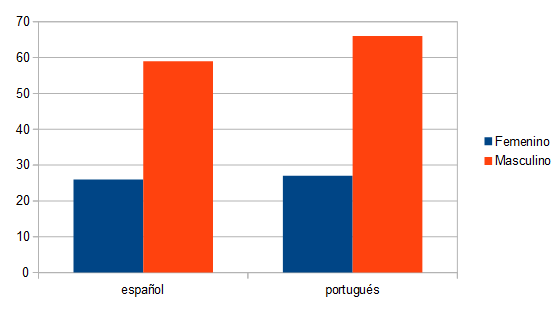
\includegraphics[width=10cm]{images/corpus/estadisticaFemMasc.png}}\\[0pt]
\caption{Estad\'istica de mujeres/hombres que completaron el experimento}
\label{estadistica-mf}
\end{center}
\end{figure}
%.....................................
\subsection{Procedimiento}
%.....................................
\label{corpus-metodo}

Las personas voluntarias recibieron un link a la interfaz del experimento, como se muestra en la Figura~\ref{fig_pagPrincipal_seleccion_idioma} esa p\'agina conten\'{i}a las instrucciones en 3 idiomas: ingl\'es, portugu\'es y espa\~{n}ol, y un link para completar el experimento en el idioma seleccionado, luego de seleccionar el idioma se mostraba la siguiente p\'agina, que recolectaba informaci\'on demogr\'afica, luego se mostraban los t\'erminos y condiciones \footnote{%
    ``Acepto de que los datos ingresados en este cuestionario sean usados an\'onimamente para investigaci\'on''
  }. 
\begin{figure}[ht]
\begin{center}
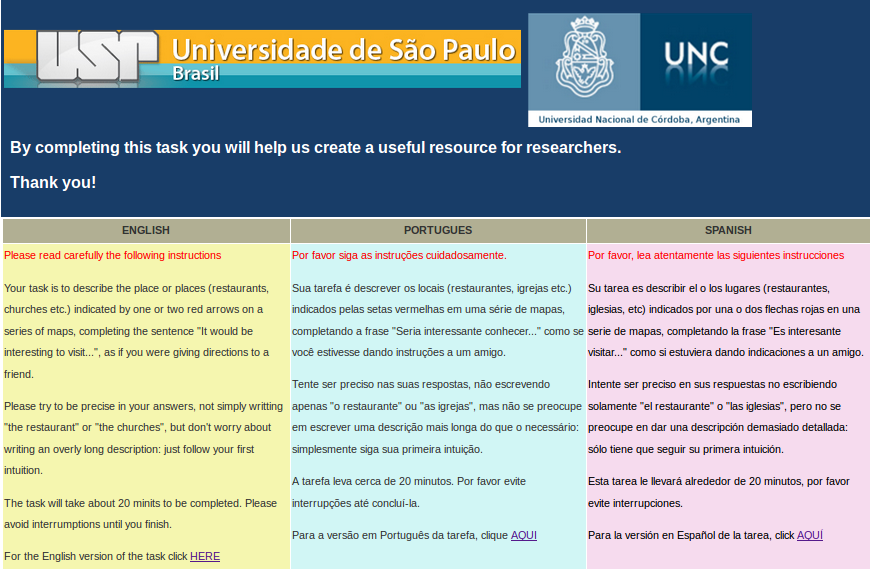
\includegraphics[width=17cm]{images/pagPrincipal.png}\\[0pt]
\caption{Link del experimento}
\label{fig_pagPrincipal_seleccion_idioma}
\end{center}
\end{figure}

Si la persona completaba los datos y aceptaba los t\'erminos y condiciones, se comenzaba el experimento mostrando, por ejemplo, la Figura~\ref{fig_interface} que tambi\'en conten\'{i}a las instrucciones, con solo pasar el mouse por la palabra instrucciones se mostraban las mismas.

\begin{figure}[ht]
\begin{center}
\frame{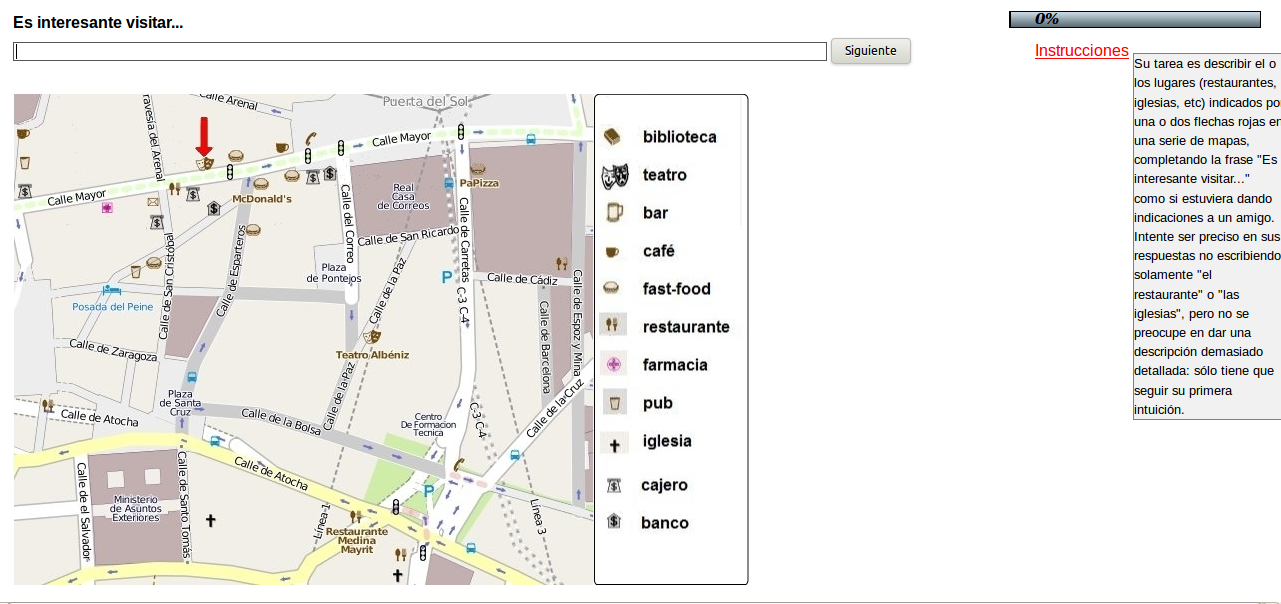
\includegraphics[width=17cm]{images/primerImagen.png}}\\[0pt]
\caption{Interface del experimento}
\label{fig_interface}
\end{center}
\end{figure}

%Las instrucciones dec\'ian lo siguiente:\\
%``Su tarea es describir el o los lugares (restaurantes, iglesias, etc) indicados por una o dos flechas rojas en una serie de mapas, completando la frase; ``Es interesante visitar...'' como si estuviera dando indicaciones a un amigo. Intente ser preciso en sus respuestas no escribiendo solamente ``el restaurante'' o ``las iglesias'', pero no se preocupe en dar una descripci\'on demasiado detallada: s\'olo tiene que seguir su primera intuici\'on''

 En la Figura~\ref{fig_pagPrincipal_seleccion_idioma} se ven las intrucciones en cada idioma, con ejemplos simples. Lo que se pretend\'ia con esas instrucciones era por un lado que la persona d\'e una expresi\'on referencial del objeto o los objetos se\~nalados que sea un sintagma nominal, que dicha expresi\'on fuera natural como le dar\'ia a un amigo y por otro lado, no incentivar a la gente a hacer ER ni minimales ni sobreespecificadas, es decir, conseguir una expresi\'on natural. 
El experimento ped\'ia completar la frase ``Es interesante visitar...'' porque a dicha frase le falta un sintagma nominal para ser una oraci\'on gramaticalmente completa. Como las ER se realizan como sintagmas nominales, esa fue la construcci\'on gramatical generada por casi todas las personas que completaron el experimento.
La p\'agina ten\'{i}a una barra indicadora de progreso, la cual se iba actualizando a medida que el usuario completaba ER. Los mapas fueron mostrados en forma aleatoria y al final del experimento se mostraba un mensaje de agradecimiento.
Cada mapa mostraba un lugar determinado (por ejemplo, un restaurante, pub, teatro, etc.) se\~nalado por una flecha como se ve en la Figura \ref{fig_interface}, donde el lugar se\~nalado por la flecha es un teatro (o dos flechas, en el caso de los plurales) como se ve en la Figura \ref{mapa20}, donde los lugares se\~nalados por las flechas son restaurantes. Despu\'es de completar la expresi\'on la persona deb\'ia pulsar el bot\'on Siguiente, entonces se seleccionaba otro est\'{i}mulo al azar y as\'{i} hasta el final del experimento. Las primeras 2 im\'agenes fueron mostradas s\'olo para que los participantes se sintieran familiar con el entorno del experimento y las respuestas dadas no fueron guardadas.

\begin{figure}[ht]
\begin{center}
\frame{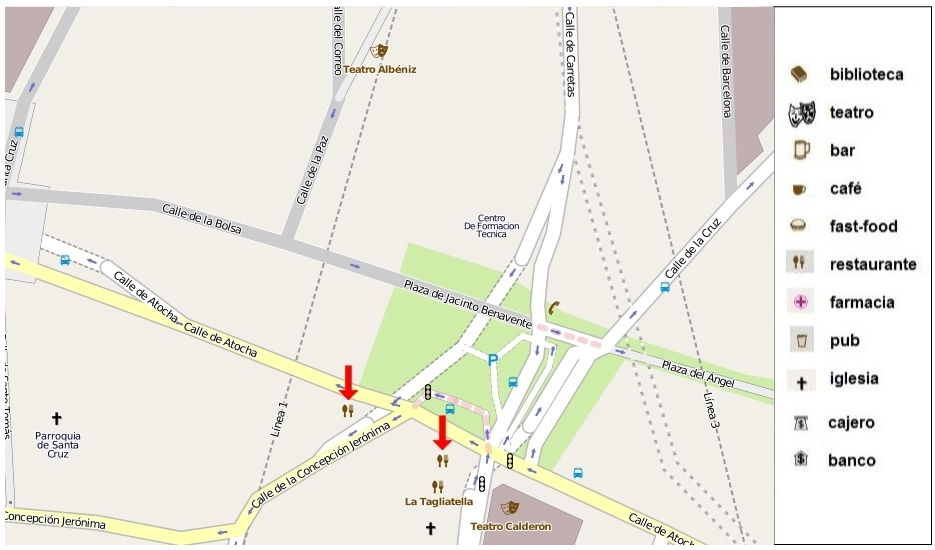
\includegraphics[width=15cm]{images/corpus/mapa20.png}}\\[0pt]
\caption{Imagen del corpus ZOOM}
\label{mapa20}
\end{center}
\end{figure}
%\hspace*{0cm}
%\begin{minipage}[b]{0.5\linewidth}
%\centering
%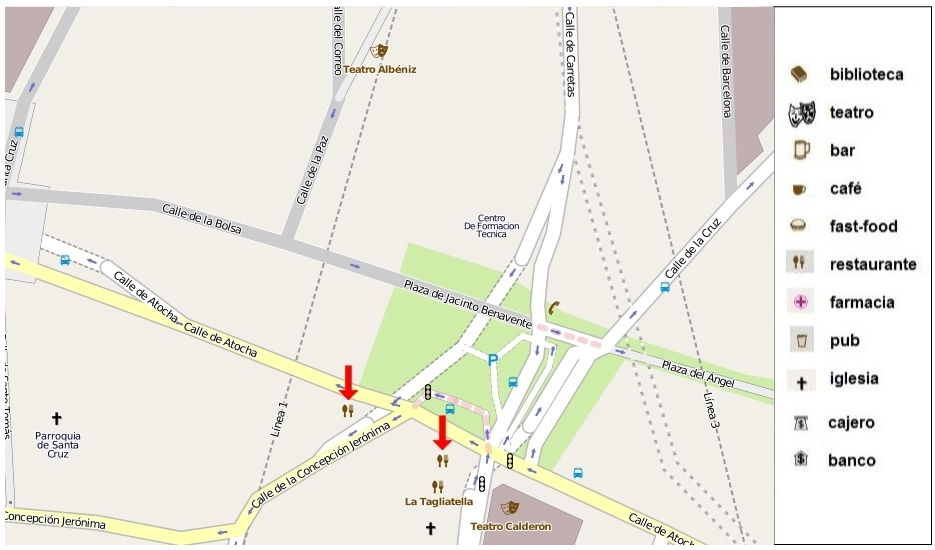
\includegraphics[width=\textwidth]{images/corpus/mapa20.png}%\\[0pt]
%\caption{Imagen del corpus ZOOM}
%\label{mapa20}
%\end{figure}

Cada vez que se presionaba el bot\'on ``Siguiente'' la p\'agina evaluaba las siguientes cosas: si hab\'ia respuesta, en el caso de no haber, aparec\'ia un cartel que dec\'ia ``Falta respuesta''.
Las descripciones mal formadas fueron descartadas siguiendo los siguientes criterios. A pesar de que las personas ten\'{i}an que completar la frase ``Es interesante visitar ...'' con un sintagma nominal que describe la ubicaci\'on se\~nalada por la flecha (o las flechas, en los casos plurales), algunas de las expresiones no eran frases nominales, sino frases completas, por ejemplo, \emph{``Vamos a ir a pizza express, es realmente barato''}, \emph{``No me gusta la comida r\'apida''}. Dichas frases fueron descartadas por no ser sintagmas nominales. Del mismo modo, se eliminaron todas las expresiones que describen un objeto que no sea el target previsto, las que utilizaban propiedades que no eran ciertas para el target, y las situaciones en que la persona ten\'{i}a que describir dos objetos pero describ\'ian s\'olo uno.



%.....................................
\subsection{Materiales}
%.....................................
\label{corpus-materiales}

El origen de los mapas usados es openstreetmaps, de ah\'i obtuvimos fragmentos de las ciudades Lisboa y Madrid. Openstreetmaps.org es una p\'agina que tiene informaci\'on de mapas de todas partes del mundo, es una organizaci\'on en la que muchas personas de distintas partes del mundo colaboran para mantener la informaci\'on actualizada. Esta informaci\'on es de libre uso, es decir uno puede usar los mapas y solo hay que nombrar de donde fueron sacados.
Se consideraron 2 idiomas: espa\~nol y portugu\'es. Se obtuvieron ER para targets singulares como se ve por ejemplo en Figuras~\ref{fig_interface} y plurales en Figuras~\ref{mapa20}, en los plurales se usaron referencias del mismo tipo (2 restaurantes, 2 iglesias, etc.) y adem\'as se tuvo en cuenta mapas con 2 niveles de zoom, X como se muestra en las (Figuras~\ref{rest-singular} y~\ref{rest-plural}) y 2X como se muestra en las (Figuras~\ref{rest-singular2x} y~\ref{rest-plural2x}). Como se puede ver en las figuras, los mapas con zoom 2X cubren una porci\'on m\'as chica de la ciudad, pero en general hay m\'as detalle.

\begin{figure}
%\begin{minipage}[b]{0.5\linewidth}
\centering
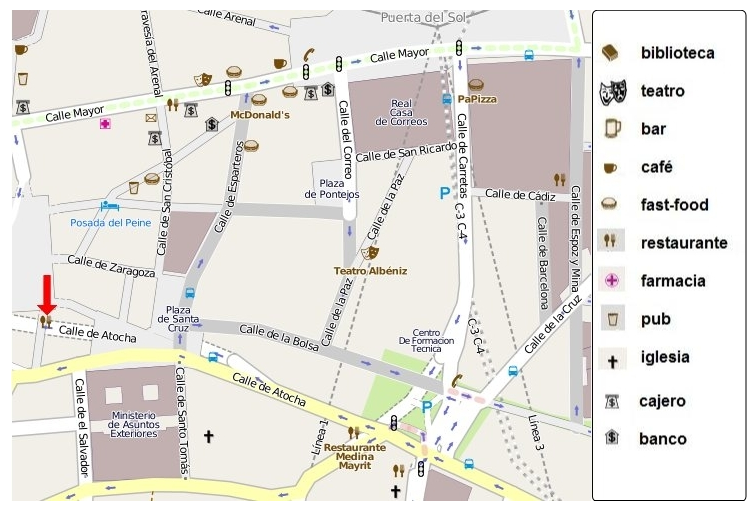
\includegraphics[width=\textwidth]{figures/rest-singular.png}\\[0pt]
\vspace*{.1cm}
\caption{Target singular con zoom X}
\label{rest-singular}
%\end{minipage}
%\hspace*{0cm}
%\begin{minipage}[b]{0.5\linewidth}
%\centering
%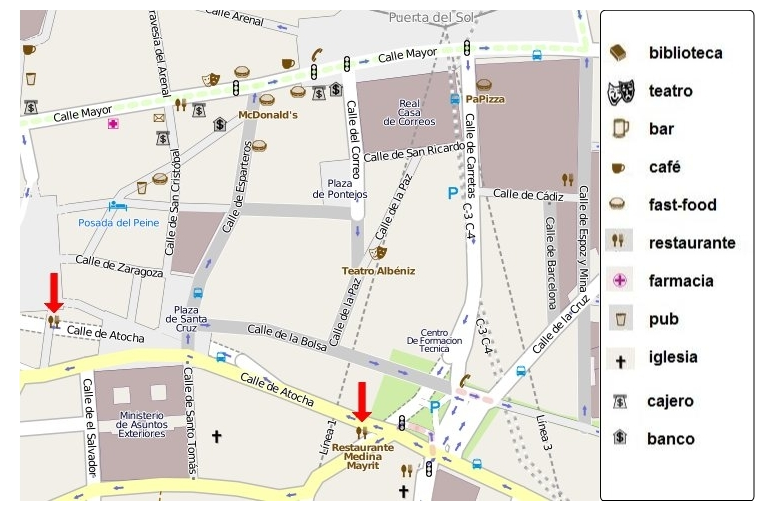
\includegraphics[width=\textwidth]{figures/rest-plural.png}\\[0pt]
%\vspace*{.1cm}
%\caption{Target plural con zoom X}
%\label{rest-plural}
%\end{minipage}
\end{figure}

\begin{figure}
\centering
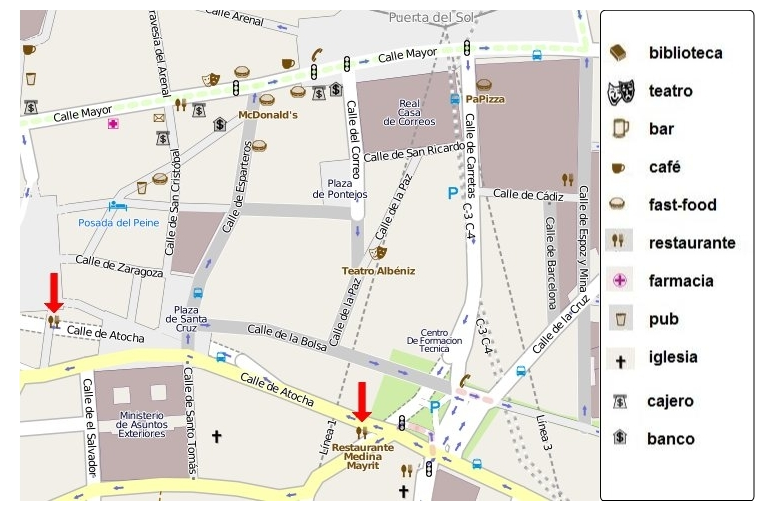
\includegraphics[width=\textwidth]{figures/rest-plural.png}\\[0pt]
\vspace*{.1cm}
\caption{Target plural con zoom X}
\label{rest-plural}
\end{figure}

\begin{figure}
%\begin{minipage}[b]{0.5\linewidth}
\centering
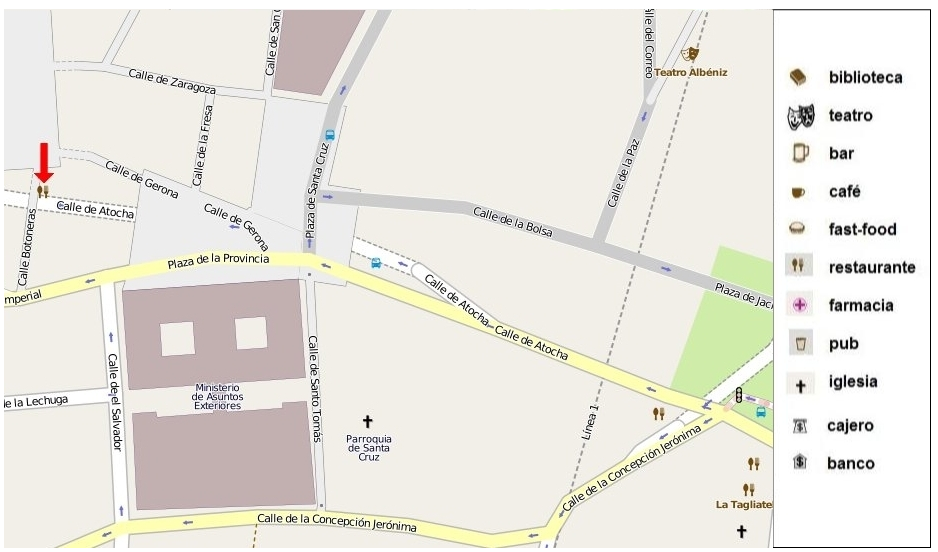
\includegraphics[width=\textwidth]{figures/rest-singular2x.png}\\[0pt]
\caption{Target singular con zoom 2X}
\label{rest-singular2x}
\end{figure}
%\end{minipage}
%\vspace*{.1cm}
%\begin{minipage}[b]{0.5\linewidth}
\begin{figure}
\centering
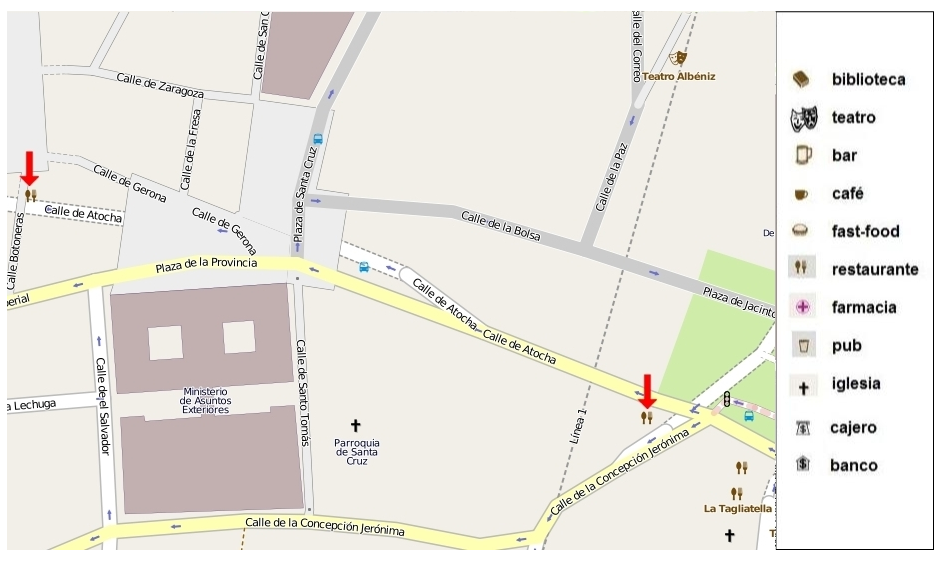
\includegraphics[width=\textwidth]{figures/rest-plural2x.png}\\[0pt]
\caption{Target plural con zoom 2X}
\label{rest-plural2x}
%\end{minipage}
\end{figure}


%El experimento hizo uso de la p\'agina especialmente dise\~nada la cual se muestra en la Figura~\ref{fig-interface}. En esa p\'agina se observa el texto ``Es interesante visitar...'', abajo hay un espacio para que la persona ingrese la expresi\'on referencial, al lado esta el bot\'on ``Siguiente'' que  al presionarlo se guardaban los datos ingresados para el est\'imulo actual y se continuaba con el siguiente est\'imulo, de el lado derecho hab\'ia una barra de estado que mostraba el progreso hasta el momento, cada vez que se presionaba el bot\'on ``Siguiente'' la barra se actualizaba llen\'andose con color verde y mostrando el porcentaje que luego de 22 mapas llegaba al 100\%, debajo del indicador de progreso hab\'ia un link que dec\'ia ``Instrucciones'', el cual al pasar el cursor del mouse desplegaba las instrucciones mostradas al inicio.
%Del lado derecho del mapa se encontraba la leyenda, que mostraba para un conjunto de \'iconos del mapa que objetos significaban, se mostraron los siguientes (biblioteca, teatro, bar, caf\'e, fast-food, restaurante, farmacia, pub, iglesia, cajero, banco), esto se realiz\'o a fin de evitar confusi\'on a las personas que daban las expresiones referenciales, ya que se not\'o por ejemplo que los \'iconos de cajero y banco podr\'ian llegar a ser identificados como la misma palabra para distintas personas. 

El mapa conten\'ia \'iconos de lugares o cosas, calles, nombres de lugares, por ejemplo podemos ver en el mapa de la Figura~\ref{fig_interface} la Calle Mayor, ah\'i se pueden ver cajeros, restaurantes, fast-foods, cafe, tel\'efonos, correos, farmacias, sem\'aforos. Notar que algunos \'iconos tienen nombre, por ejemplo el fast-food McDonald's. Algunos edificios o plazas tambi\'en tienen nombre como la Real Casa de Correos y la Plaza de Pontejos. En el mapa tambi\'en podemos ver algunos objetos sin nombre.
Se puede ver en las Figuras~\ref{rest-singular2x} y~\ref{rest-plural2x}  el nombre de la iglesia Parroquia de Santa Cruz, pero en las Figuras~\ref{rest-singular} y~\ref{rest-plural} no se muestra el nombre, se ve solamente el \'icono. Pero para el Ministerio de Asuntos Interiores se ve el nombre en ambos niveles de zoom. Notar que no siempre en el nivel 2X de zoom se ver\'a todo lo que se ve y m\'as que en el nivel X, por ejemplo tenemos el restaurante Medina Mayrit, cuyo nombre se ve en Figura~\ref{rest-singular} pero no se ve en Figura~\ref{rest-singular2x}. 
%Suponemos que esto tiene que ver con la superposici\'on de nombres, 
Los mapas eran fragmentos del centro de la ciudad de Madrid (para la parte espa\~nola del corpus) y de Lisboa (para la parte portuguesa).
Para cada ciudad, se utilizaron 10 mapas con distintas ubicaciones. Cada ubicaci\'on se muestra con un nivel X y 2X de zoom, haciendo 20 im\'agenes en total. En ambos niveles de zoom el objetivo se\~{n}alado se mantuvo.%, pero en la versi\'on m\'as detallada, por supuesto, se ve un mayor n\'umero de distractores y detalles adicionales en general. %Algunos nombres de las calles y de landmarks podi\'{i}an no aparecer en diferentes niveles de zoom.
La mitad de las im\'agenes mostraron una sola flecha que apunta a un objeto en el mapa (es decir, requer\'{i}an una sola descripci\'on como por ejemplo en la Figura~\ref{rest-singular} ``el restaurante en la Calle de Atocha, cerca del Ministerio de Asuntos Exteriores''), mientras que en la otra mitad mostr\'o dos flechas que apuntaban a dos lugares diferentes (y por lo tanto requer\'ian una referencia a un conjunto, como en Figura~\ref{rest-plural} ``los dos restaurantes de la Calle de Atocha'' o ``el restaurante cerca del Ministerio de Asuntos Exteriores y el Medina Mayrit'').


\subsection{Datos recolectados}
\label{sec:datos_recolectados}

La p\'agina web del experimento se mantuvo en l\'{i}nea hasta que se obtuvieron 100 experimentos completos para el portugu\'es y 85  para el espa\~nol. Luego de la verificaci\'on manual, se descartaron 602 descripciones portuguesas mal formadas y 366 descripciones espa\~nolas. As\'{i}, la parte portuguesa del corpus consta de 1.358 descripciones mientras que la parte espa\~nola contiene 1.234 ER. La p\'agina fue inicialmente pensada para obtener el corpus en 3 idiomas, pero luego se recolect\'o s\'olo en 2: espa\~nol y portugu\'es. La p\'agina sigue en l\'inea, y el c\'odigo de la misma est\'a disponible por si a alguien le interesa recolectar un corpus similar.
\footnote{http://cs.famaf.unc.edu.ar/~romina/pagina/}
%En la Secci\'on~\ref{sec-problemas} se describen los criterios por los que se consideraron las descripciones mal formada.\textcolor{blue}{de esto ya hable antes...} Tambi\'en se discuten el desaf\'{i}o que supone obtener las ER en lenguaje natural en un experimento basado en la web para un dominio que es significativamente m\'as cerca de aplicaciones del mundo real que los corpus GER existentes.
En la parte portuguesa de los datos, el 78,6\% de las descripciones incluyen propiedades relacionales. Adem\'as de eso, el 36,4\% eran minimales un 44,3\% eran sobreespecificadas, y el 19,3\% eran subespecificadas. En la parte espa\~nola de los datos, 70\% de las descripciones incluyeron propiedades relacionales. Por otra parte, el 35\% eran minimales, el 40\% eran sobreespecificadas, y el 25\% eran subespecificadas.
Esta proporci\'on tan grande de descripciones subespecificadas as\'{i} como descripciones relacionales no son comunes en corpora GER existente (o por lo menos en tal proporci\'on), esto puede reflejar la complejidad del dominio o limitaciones en el entorno web en el cual se bas\'o la obtenci\'on del corpus.



\subsection{Anotaci\'on del corpus}
\label{corpus-anotacion}

\begin{figure}[H]
\centering
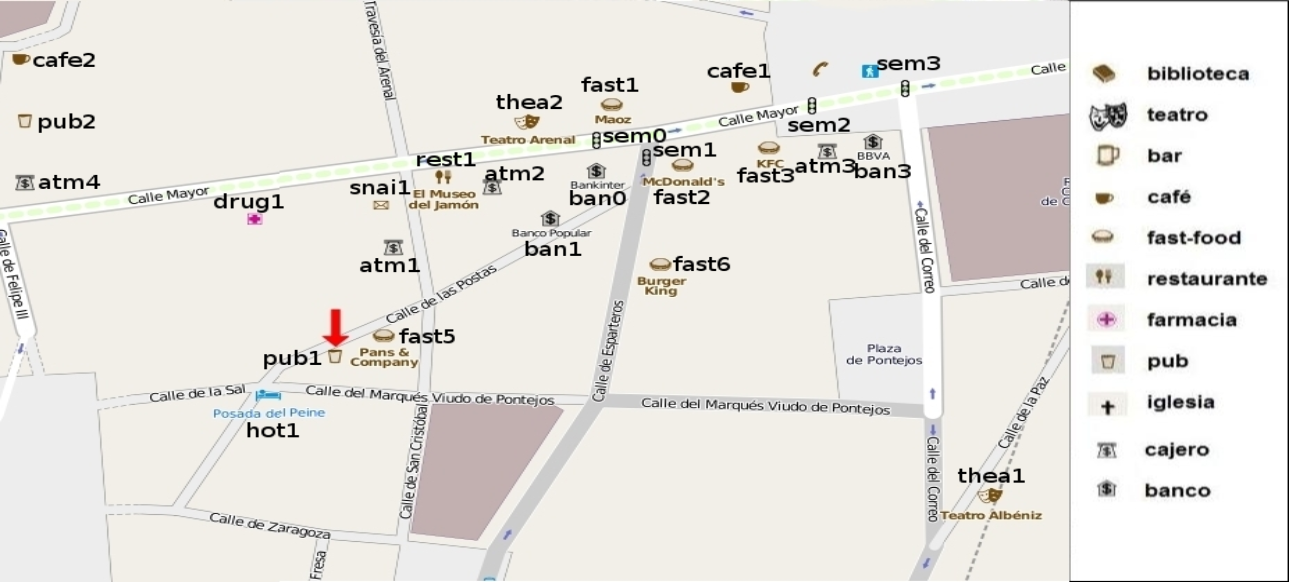
\includegraphics[width=\textwidth]{figures/mapa-con-ids2.png}\\[0pt]
\caption{Mapa con Id's usado para la anotaci\'on}
\label{mapa-con-ids}
\end{figure}

\begin{table}[!t]
{\footnotesize
\begin{center}
\begin{tabular}{|l|r|r|r|}
\hline
Tipo & Nombre & En & ID\\
\hline

cafe & & & cafe2 \\
pub	& & & pub2 \\
atm	& & str1 & atm4 \\
drugstore & & str1 & drug1\\
snailpost & & str1,str2 & snai1\\
restaurant & el museo del jamon & str1,str2 & rest1\\
atm	& & str1 & atm2\\
theater & & str1 & thea2\\
semaphore & & str1 & sem1\\
semaphore & & str1 & sem2\\
semaphore & & str1,str3 & sem3\\
fast-food & maoz & str1 & fast1\\
fast-food & mcdonalds & str1,str4 & fast2\\
fast-food & kfc & str1 & fast3\\
cafe & & str1 & cafe1\\
fast-food & burger king & str4 & fast6\\
atm	& & str1 & atm3\\
pub	& & str1,str3 & ban3\\
fast-food & pans and company & str2 & fast5\\
pub	& & str15 & pub1\\
hotel & posada del peine & str15,str19 & hot1\\
bank & banco popular & str15 & ban1\\
semaphore & & str1,str5 & rest5\\
fast-food & papizza & str5 & fast4\\
restaurant	& & str6,str7 & rest5\\
theater	& & str8 & thea1\\
semaphore & & str9 & sem5\\
semaphore & & str9 & sem6\\
restaurant & & str9 & rest2\\
church	& & str9,str10 & chur1\\
restaurant & medina mayrit & str9 & rest3\\
restaurant & & str9 & rest4\\
church & & str11 & chur2\\
bank & bankinter & str15 & ban0\\
street & calle mayor & & str1 \\
street & calle de san cristobal & & str2\\
street & calle del correo & & str3\\
street & calle de esparteros & & str4\\
street & calle de carretas & & str5\\
street & calle de espoz y mina & & str6\\
street & calle de cadiz & & str7\\
street & calle de la paz & & str8\\
street & calle de antocha & & str9\\
street & calle de santo tomas & & str10\\
street & calle de la cruz & & str11\\
street & calle del salvador & & str12\\
street & calle de la bolsa & & str13\\
street & calle de zaragoza & & str14\\
street & calle de las postas & & str15\\
street & calle botoneras & & str16\\
street & calle de gerona & & str17\\
street & calle de la sal & & str18\\
street & calle del marquez viudo de pontejos & & str19\\
\hline
\end{tabular}
\caption{Objetos identificados de la Figura~\ref{mapa-con-ids}\label{tabla-ids}}
\vspace*{-.5cm}
\end{center}
%\end{small}
}
\end{table}

Para cada imagen se construy\'o una tabla con los id's de los objetos que se ven, como por ejemplo para la imagen~\ref{mapa-con-ids} la tabla correspondiente es la Tabla~\ref{tabla-ids} al mapa se le agregaron los id's de algunos objetos del mapa, estos identificadores eran \'unicos. Por ejemplo {\it pub1} es el que esta siendo apuntado por la fecha roja en la Figura~\ref{mapa-con-ids}. A cada calle tambi\'en se le asign\'o un identificador \'unico pero estos se anotaron en una tabla, como se ve en la Tabla~\ref{tabla-ids}. Dicha tabla tiene 4 columnas para cada objeto se puso ``tipo'', ``nombre'', ``en'' y ``id'', el tipo es por ejemplo, restaurante, bar, street (estos nombres de tipos se pusieron en Ingl\'es), ``nombre'', el nombre propio del objeto, si ten\'ia, (se mantuvieron en el idioma original, espa\~nol o portugu\'es), ``en'', conten\'ia la calle en la que estaba situado el objeto, y si era una calle no conten\'ia nada e ``id'' que fue compuesto por 3 o 4 primeras letras del tipo del objeto m\'as un n\'umero para identificarlo un\'ivocamente, por ejemplo para los restaurantes ``rest1'', ``rest2''.

%- Los valores de los atributos se anotaron en Ingl\'es (por ejemplo, restaurant, pub, street, etc.), pero los nombres propios (para calles, etc.) se mantuvieron en su forma original, tal cual se v\'e en el mapa (Espa\~{n}ol, Portugu\'es).

Se seleccion\'o un conjunto fijo de atributos para cada objeto, pero dando flexibilidad con un atributo llamado ``other'' que permit\'ia anotar otras cosas que hayan aparecido en la expresi\'on dada por la persona, que no estuviera en la lista fija. En esta manera de anotar, cada objeto tiene como m\'aximo 26 posibles atributos.

En el caso de las descripciones plurales, el conjunto de atributos se repite para cada objeto, por lo que el anotador pod\'{i}a utilizar hasta 52 atributos.

Los 26 o 52 atributos nombrados anteriormente estan formados por:
10 atributos que denotan caracter\'isticas del objeto principal (target), o relaciones que pueden tener 1 o 2 par\'ametros como en el caso de en-frente-de, el cual toma como par\'ametro un id de objeto:
\begin{itemize}
  \item tipo (por ejemplo, restaurante)
  \item nombre (por ejemplo, McDonalds)
  \item en (calle-id, avenida-id, etc.)
  \item izquierda (obj-id)
  \item derecha (obj-id)
  \item en esquina / entre (Street1, Street2)
  \item cerca (obj-id)
  \item en-frente-de (obj-id)
  \item detr\'as (obj-id)
  \item otro (cualquier otra cosa mencionada en la descripci\'on, pod\'ia ser una propiedad o relaci\'on)
\end{itemize}
y 16 atributos que denotan los objetos adicionales (landmarks) que se mencionaron en la descripci\'on, a los cuales llamamos d1..d4. Por ejemplo, en ``El pub que esta al lado de Pans \& Company, en la Calle de las Postas'') tenemos:target = pub, d1 = fast-food (Pans \& Company) y d2 = Street (Calle de las Postas).\\

Para cada target se consider\'o un m\'aximo 4 objetos tomados como puntos de referencia (landmarks), ya que con esta cantidad cubr\'iamos las descripciones m\'as largas y se anotaron como d1..d4, para cada landmark se anotaron 4 atributos:
\begin{itemize}
  \item Identificaci\'on (Id)
  \item Tipo (un sustantivo, restaurant, pub...)
  \item Nombre
  \item Otro (alguna otra cosa dicha sobre el objeto)
\end{itemize}

A su vez cada atributo tiene una lista estricta de los valores permitidos. Por ejemplo, para el objetivo de la Figura~\ref{mapa-con-ids} los valores posibles para el tipo de atributo son s\'olo dos:``pub'' u ``otro''. El valor ``otro'' le da al anotador una oportunidad de dar una respuesta cuando la descripci\'on muestra algo muy inusual.

Para los atributos espaciales (izquierda, cerca, etc.) permitimos que los valores que denota la mayor\'{i}a de los objetos en el mapa, a excepci\'on de aquellos que son claramente ilegales. Por ejemplo, en el caso de la ``izquierda'' posibles valores incluyen la mayor\'{i}a de los objetos en la pantalla, a excepci\'on de los de la derecha del objeto target. Por ejemplo, para el objetivo de la Figura~\ref{mapa-con-ids} es posible decir ``el pub que esta a la izquierda de Pans \& Company'', pero no es admitido ``El pub que esta a la izquierda de Posada del Peine''.
%MOVER A OTRO LADO ESTA SECCION
%
%%%%%%%%%%%%%%%%%%%%%%%%%%%%%%%%%%%%%%%%%%%%%%%%%%%%%%%%%%%%%%%%%%%%%%%%%%%%%%%%%%%%%%%%%%%%%%%%%%%%%%%%%%%%%%%%%%%%%%%%%%%%%%%%%%%%%%%%%%%%%%%%%%%%%%%%%	       
%\section{Background}
%%%%%%%%%%%%%%%%%%%%%%%%%%%%%%%%%%%%%%%%%%%%%%%%%%%%%%%%%%%%%%%%%%%%%%%%%%%%%%%%%%%%%%%%%%%%%%%%%%%%%%%%%%%%%%%%%%%%%%%%%%%%%%%%%%%%%%%%%%%%%%%%%%%%%%%%%%	       
%\label{sec-background}

%In this section we briefly discuss a number of GER corpora publicly available for research purposes, and how these resources compare to our current work.

%TUNA \cite{tuna-corpus} was the first prominent GER corpus to be made publicly available for research purposes. The corpus was developed in a series of general-purpose controlled experiments, containing 2280 descriptions produced by 60 speakers in two domains (1200 descriptions of furniture items and 1080 descriptions of people's photographs). TUNA does not contain relational descriptions, and it is possibly the only resource of this kind to include situations of reference to sets. The TUNA corpus has been extensively used in a series of shared tasks \cite{reg2009}.

%TUNA \cite{tuna-corpus} fue el primer prominente corpus GER para estar disponible al p\'ublico para fines de investigaci\'on. El corpus fue desarrollado en una serie de experimentos controlados de prop\'osito general, que contiene 2.280 descripciones producidas por 60 altavoces en dos dominios (1.200 descripciones de art\'{i}culos de los muebles y 1080 en las descripciones de las fotograf\'{i}as de las personas). AT\'UN no contiene descripciones relacionales, y es posiblemente el \'unico recurso de este tipo para incluir situaciones de referencia a los conjuntos. El corpus AT\'UN se ha utilizado ampliamente en una serie de tareas compartidas \cite{reg2009}.



%GRE3D3 and its extension GRE3D7 \cite{gre3d3,gre3d7} were developed in a series of web-based experiments primarily focussed on the study of relational descriptions. GRE3D3 contains 630 descriptions produced by 63 speakers, and GRE3D7 contains 4480 descriptions produced by 287 speakers, making it the largest of its kind to date. The GRE3D domain consists of simple visual scenes containing only two kinds of objects (boxes and spheres) with limited variation in colour and size. In each scene, there is only one possible spatial relation between target and the nearest landmark. Both corpora contain atomic and relational descriptions.


%GRE3D3 and its extension GRE3D7 \cite{gre3d3,gre3d7}
%se desarrollaron en una serie de experimentos basados en la Web se centraron principalmente en el estudio de las descripciones relacionales. GRE3D3 contiene 630 descripciones producidas por 63 altavoces, y GRE3D7 contiene 4.480 descripciones producidas por 287 oradores, por lo que es el mayor de su tipo hasta la fecha. El dominio GRE3D consta de escenas visuales simples que contienen s\'olo dos tipos de objetos (cajas y esferas) con variaci\'on limitada en color y tama\~no. En cada escena, s\'olo hay una posible relaci\'on espacial entre el objetivo y el hito m\'as cercano. Ambos cuerpos contienen descripciones at\'omicas y relacionales.

%Stars \cite{stars-mutual-disamb} and its extension Stars2 were collected for the study of referential overspecification (particularly in the case of relational descriptions). Stars was developed in a pilot web-based experiment, containing 704 descriptions produced by 64 speakers.  The more comprehensive Stars2 data set was produced in dialogue situations involving subject pairs, and it contains 884 descriptions produced by 56 speakers. Both domains make use of simple visual scenes containing up to four object types (e.g., stars, boxes, cones and spheres) with limited variation in colour and size. Differently from other GER corpora, however, Stars/2 includes a considerable number of complex situations of reference involving up to three objects, as in `the box near the sphere, next to the cone'. 


%Stars \cite{stars-mutual-disamb} y su extensi\'on Stars2 se recogieron para el estudio de sobrevaloraci\'on referencial (particularmente en el caso de las descripciones relacionales). Estrellas se desarroll\'o en un experimento basado en la web piloto, que contiene 704 descripciones producidas por 64 altavoces. El conjunto de datos Stars2 m\'as completa se produjo en situaciones de di\'alogo que implican pares sujetos, y contiene 884 descripciones producidas por 56 altavoces. Ambos dominios hacen uso de escenas visuales simples que contienen hasta cuatro tipos de objetos (por ejemplo, estrellas, cajas, conos y esferas) con variaci\'on limitada en color y tama\~no. A diferencia de otros GER corpus, sin embargo, Estrellas / 2 incluye un n\'umero considerable de situaciones complejas de referencia que incluyan hasta tres objetos, como en `la caja cerca de la esfera, al lado del cono".


%Despite their usefulness and general contribution to the research in REG, the above domains are still at a certain distance from the kinds of visual scene that might be required for a practical, real-world application. The need for additional complexity and/or realism, and our own interest in the surface realisation task for the Spanish and Portuguese languages, has led us to build a new computational resource of this kind. This work is described in the next sections. Further discussion on the differences between the Zoom corpus and existing resources is presented in Sec. 


%A pesar de su utilidad y contribuci\'on general a la investigaci\'on en REG, los dominios anteriores se encuentran todav\'{i}a en una cierta distancia de los tipos de escena visual que podr\'{i}an ser necesarias para una aplicaci\'on en el mundo real pr\'actico. La necesidad de complejidad y / o realismo adicional, y nuestro propio inter\'es en la tarea realizaci\'on de superficie para los idiomas espa\~nol y portugu\'es, nos ha llevado a construir un nuevo recurso computacional de este tipo. Este trabajo se describe en las siguientes secciones. Continuaci\'on del debate sobre las diferencias entre el corpus Zoom y los recursos existentes se presenta en la Sec.\ref{sec-annotation}. 



%.....................................
%\subsection{El corpus y la anotaci\'on}
%.....................................
%\label{sec-annotation}

%The experiment website was kept online until 100 complete trials were obtained for Portuguese and 80 complete trials were obtained for Spanish. Upon manual verification, 602 ill-formed Portuguese descriptions and 366 Spanish descriptions were discarded. Thus, the Portuguese portion of the corpus consists of 1358 descriptions while the Spanish portion contains 1234 referring expressions. In Section~\ref{sec-problems} we describe the criteria by which descriptions were considered ill-formed. We also discuss the challenges faced when collecting natural language descriptions in a web-based experiment for a domain that is significantly closer to real-world applications than existing GER corpora. 

%In the Portuguese portion of the data, 78.6\% of the descriptions include relational properties. In addition to that, 36.4\% were minimally distinguishing, 44.3\% were overspecified, and  19.3\% were underspecified. In the Spanish portion of the data, 70\% of the descriptions include relational properties. Moreover, 35\% were minimally distinguishing, 40\% were overspecified, and 25\% were underspecified. Underspecified descriptions as well as relational descriptions are not common in existing GER corpora - certainly not in this proportion.  

%Table \ref{tab-comparison} presents a comparison between the collected data and existing GER corpora. The domain information represents the number of possible atomic attributes and the number of relations in each description. The information on TUNA and Zoom descriptions is based on the singular portion of each corpus only. This represents the average description size (in number of annotated properties) and properties usage, which is taken to be  the proportion of properties that appear in the description over the total number of possible attributes and landmarks. From a GER perspective, larger description sizes and lower usage scores are likely to represent more complex situations of reference.

%IP:I realise that what I meant to show here was not the number of possible relations in each corpus (which in some cases is very large - below, above, near, nextto, etc.) but simply the maximum number of relations that may appear in each description. This is the same as reporting the number of landmark objects in addition to the main target. I fixed this now by changing the text and column title to ``landmarks', and I also updated the Zoom rows from 7 relations to 4 landmarks. The data regarding the other corpora was already reflecting the number of landmarks rather than the number of relations, so no further changes were required.





%Annotation was performed as follows. Each referring expression was modelled as conveying a description of the main target object and, optionally, up to four descriptions of related landmarks. The annotation scheme consisted of three target attributes, four landmark attributes for each of the four possible landmark objects, and seven relational properties. This makes 26 possible attributes for each referring expression. In the case of plural descriptions (i.e., those involving two target objects), this attribute set is doubled.

%Every object was annotated with the atomic attributes {\em type}, {\em name} and {\em others} and, in the case of landmark objects, also with their {\em id}. In addition to that, seven relational properties were considered:{\em in/on/at}\footnote{The three prepositions were aggregated as a single attribute because they have approximately the same meaning in the languages under consideration}, {\em next-to}, {\em right-of}, {\em left-of}, {\em in-front-of}, {\em behind-of}, and the multivalue relation {\em between} intended to represent `corner' relations. 

%Possible values for the {\em type} and {\em name} attributes are predefined by each referential context. The {\em others} attribute may be assigned any string value, and it is intended to represent any non-standard piece of information conveyed by the referring expression. For the spatial relations, possible values are the object identifiers available from each scene.

%The collected descriptions were fully annotated by two independent annotators. After completion, a third annotator assumed the role of judge and provided the final annotation. Since the annotation scheme was fairly straightforward (i.e., largely because all non-standard responses were simply assigned to the {\em others} attribute), agreement between judges as measured by Kappa \cite{kappa} was 84\% at the attribute level. 

%Both referential contexts and referring expressions were represented in XML format using a simplified version of the XML format adopted in the TUNA corpus \cite{tuna-corpus}. Descriptions were grouped into TRIAL nodes containing general information about each subject (i.e., id, age and gender) followed by his/her list of responses. Each response identifies the context within which it was produced, and the referring expression proper. 

%As in \cite{tuna-corpus}, the contents of referring expressions are represented by ATTRIBUTE-SET nodes containing a list of attribute names and their values. The following example illustrates a fragment of this representation for an elicited description. Objects in each input context were represented in a similar fashion.

%La anotaci\'on se realiz\'o como sigue. Cada ER da una descripci\'on del objeto target y, opcionalmente, hasta cuatro descripciones de landmarks relacionados. El esquema de anotaci\'on consisti\'o en tres atributos para el target, cuatro atributos para cada uno de los cuatro posibles landmarks, y siete propiedades relacionales. Esto hace 26 posibles atributos para cada expresi\'on referencial. En el caso de las descripciones plurales (es decir, los que implican dos objetos se\~{n}alados), este conjunto de atributos se duplica.

%Cada objeto fue anotado con los atributos at\'omicos {\em tipo}, {\em nombre} y {\em otros} y, en el caso de objetos landmarks, tambi\'en con su {\em Identificaci\'on}. Adem\'as de eso, se consideraron siete propiedades relacionales:{\em en / sobre / a} \footnote{Las tres preposiciones fueron agregadas como un \'unico atributo, ya que tienen aproximadamente el mismo significado en los idiomas considerados}, {\em pr\'oximo -para}, {\em derecho-de}, {\em izquierda de}, {\em en-frente-de}, {\em detr\'as de}, y la relaci\'on {\em entre} que pretende representar relaciones `esquina'.


%Los valores posibles para los atributos {\em tipo} y {\em nombre} est\'an predefinidos por cada contexto referencial. En el atributo {\em otros} puede asignar cualquier valor de cadena, y se pretende representar cualquier pieza no est\'andar de la informaci\'on transmitida por la ER. Para las relaciones espaciales, los valores posibles son los identificadores de los objetos disponibles en cada escena.

Las descripciones recolectadas fueron totalmente anotadas por dos anotadores independientes. Luego, un tercer anotador asumi\'o el rol de juez y di\'o la anotaci\'on final. Dado que el esquema de anotaci\'on fue bastante sencillo (es decir, en gran parte porque las respuestas no estandares simplemente se asignan al atributo {\em otros}), se midi\'o el acuerdo entre los jueces, con Kappa \cite{kappa}, \'este fue del 84\% en el nivel de atributo.
Ambos, el contexto y las ER estuvieron representados en formato XML utilizando una versi\'on simplificada del formato XML adoptado en el corpus TUNA \cite{tuna-corpus}. Las descripciones se agruparon en nodos TRIAL que contienen informaci\'on general sobre cada persona (es decir, identificaci\'on, edad y sexo), seguido de su lista de respuestas. Cada respuesta identifica el contexto en que se produjo, y la expresi\'on en referencial que la persona dijo.
Al igual que en \cite{tuna-corpus}, el contenido de las expresiones referenciales est\'an representadas por nodos que son conjunto de atributos que contienen una lista de nombres de atributos y sus valores. El siguiente ejemplo ilustra un fragmento de esta representaci\'on para una ER. Los objetos en cada contexto de entrada estaban representados de una manera similar.
Para el target de la Figura~\ref{mapa-con-ids} y la expresi\'on ``El pub que esta al lado de Pans \& Company, en la
Calle de las Postas'', la anotaci\'on ser\'ia la siguiente.
%\tiny{
\begin{verbatim}
<TRIAL ID="2" SPEAKER="166" AGE="18" GENDER="m">
  <CONTEXT ID="3" SEQ="1300">
     <ATTRIBUTE-SET TARGET="pub1" LANDMARK="fast5" 
                    STRING="El pub que esta al lado de Pans & Company, 
                            en la Calle de las Postas">
        <ATTRIBUTE NAME="type" VALUE="pub" />
        <ATTRIBUTE NAME="at" VALUE="str15" />
        <ATTRIBUTE NAME="landmark-name" VALUE="Pans & Company" />
     </ATTRIBUTE-SET>
  </CONTEXT>
</TRIAL>	
\end{verbatim}
%}
%\normalsize


%In each description, attribute names for the first landmark object are preceded by the `landmark-' label as in the above example. Subsequent landmarks were labelled as `second-landmark' and so on. This was motivated by the need to provide unique attribute names for the benefit of GER algorithms.

%The set of images, text descriptions and their XML representations constitutes the Zoom corpus of referring expressions, to be made publicly available for research purposes. As a first step in this direction, the following sections present the results of a machine learning approach to GER based on the Portuguese portion of the data.

En cada descripci\'on, el nombre para el primer landmark es el VALUE del ATTRIBUTE con NAME `landmark-name' como en el ejemplo anterior. Los landmarks siguientes fueron etiquetados como ``second-landmark'' y as\'{i} sucesivamente. Esto fue motivado por la necesidad de proporcionar nombres de atributos \'unicos para el beneficio de los algoritmos GER.
El conjunto de im\'agenes, textos descriptivos y sus representaciones XML constituye el corpus ZOOM de ER, el cual ser\'a p\'ublico para fines de investigaci\'on. Como primer paso en esta direcci\'on, las siguientes secciones se presentan los resultados de un enfoque de aprendizaje autom\'atico para GER, los cuales se basan en la parte portuguesa del corpus.

\subsection{Comparaci\'on con trabajo previo}
\label{sec:comparacion_trabajo_previo}

En la Tabla~\ref{tab-comparison} se presenta una comparaci\'on entre el corpus recolectado y otros corpus de RE existentes nombrados en~\ref{sec:corpus-existente}. La informaci\'on de dominio representa el n\'umero de posibles atributos at\'omicos y el n\'umero de relaciones en cada descripci\'on. La informaci\'on sobre el TUNA-corpus y las descripciones de ZOOM se basan s\'olo en la parte singular de cada corpus. Esto representa el tama\~no medio de la descripci\'on (en n\'umero de propiedades anotadas) y la utilizaci\'on de las propiedades, la cual se toma como la proporci\'on de las propiedades que aparecen en la descripci\'on sobre el n\'umero total de posibles atributos y puntos de referencia.\textcolor{blue}{reescribir- Desde una perspectiva de GER, las ER de mayor tama\~no y las puntuaciones m\'as bajas de uso es probable que representen las situaciones m\'as complejas de referencia.}


\begin{table}[H]
\begin{center}
\footnotesize{
\caption{Comparaci\'on con corpus de GER existente}
\label{tab-comparison}
\begin{tabular} {  l c c c c}
\hline
%\multicolumn{1}{c}{}
%&\multicolumn{1}{c}{Domain}
%&\multicolumn{3}{c}{Descriptions}\\
Corpus											& Atributos			& Landmarks			& Tama\~{n}o promedio	& Uso \\
\hline
TUNA-Furniture							& 4								& 0							& 3.1				& 0.8   \\
TUNA-People									& 10							& 0							& 3.1				& 0.3   \\
GRE3D3											& 9								& 1							& 3.4				& 0.3   \\
GRE3D7											& 6								& 1							& 3.0				& 0.4   \\
Stars												& 8								& 2							& 4.4				& 0.4   \\
Stars2											& 9								& 2							& 3.3				& 0.3   \\
Zoom-Pt											& 19							& 4							& 6.7				& 0.3   \\
Zoom-Sp											& 19							& 4							& 7.2				& 0.3   \\
\hline
\end{tabular}
}
\end{center}
\end{table}
%.....................................
\subsection{Discusi\'on}
%.....................................
\label{corpus-discusion}

%Previous corpora of referring expressions have been collected in specially designed and highly controlled domains. Collecting corpora from a domain that is directly relevant to real-world applications poses a significant challenge not only to the collection and annotation process itself but also to existing GER algorithms. This is made evident by the large proportion of referring expressions that needed to be manually discarded from our dataset because the did not constitute a referring expression of the intended target. This proportion is 30\% for the Portuguese portion of the dataset and 23\% for the Spanish portion. 

%The ill-formed descriptions were discarded following the criteria that we explain here. As seen in Figura~\ref{fig-interface} subjects had to complete the sentence ``It would be interesting to visit ...'' with a noun phrase describing the location signalled by the arrow. However, some of the referring expressions were not noun phrases but full sentences. For example, responses such as ``Let's go to pizza express, it's really cheap'' were discarded because the subject had in mind a communicative goal other than identifying the target. Moreover, a few subjects completed the experiment with sentences like ``I don't like fast food'' which were clearly out of domain. Similarly, we removed all expressions that described an object other than the intended target, which used properties that were not true of the target, all situations in which the subject had to describe two objects but described only one, and all descriptions containing only the basic attribute type (as in ``the church'').

%After this cleaning process the Portuguese portion of the corpus still contains a 19.3\% of underspecified referring expressions and the Spanish portion a 25\%. An example of underspecified referring expression is shown in Figura~\ref{fig-interface}; the referring expression ``the pub at Cowgate'' is underspecified because there are two pubs at Cowgate street on the map. The percentage of underspecified referring expressions in the Zoom corpus is much higher than that reported in the corpora described in the the previous section, which is not higher than 5\%. Previous psycholinguistic studies~\cite{Clark1986} have found that over 20\% of the referring expressions in naturally occurring discourse are underspecified with respect to the established context. In sufficiently complex domains,~\cite{Clark1986} found that speakers will often produce an initial underspecified referring expression, and then repair it if necessary instead of producing a uniquely identifying description from the start. As discussed in 
%the previous section, the Zoom domain is likely contain more complex situations of reference if compared to existing resources of this kind, that is,  Zoom description are on average longer, and have a lower average attribute usage. This, in our opinion, may explain the high proportion of referential underspecification in our data.   

%The proportion of overspecified referring expressions of the Zoom corpus is similar to that found in previous work. However, the proportion of relational descriptions is presently higher. Relational descriptions constitute a challenge for GER algorithms due to the computational complexity associated to their generation~\cite{survey}. A further challenge posed by the Zoom corpus is the fact that it contains two descriptions for every target based on different - but related - models corresponding to the same map location seen with different zoom levels. For instance a map with higher zoom level (2X) is illustrated in Figura~\ref{fig-with-zoom}, and the same map with lower zoom level is shown in Figura~\ref{fig-interface}. 


Corpora anterior de expresiones referenciales se han recogido en los dominios de dise\~no especial y muy controladas. 

La recopilaci\'on de corpus de un dominio que es directamente relevante para aplicaciones del mundo real plantea un reto importante no s\'olo para el proceso de recolecci\'on y anotaci\'on en s\'{i}, sino tambi\'en a los algoritmos GER existentes. Esto se hace evidente por la gran proporci\'on de las expresiones referenciales que deben ser desechadas desde nuestra base de datos porque no constituyen una ER para el objeto target. Esta proporci\'on es del 30\% de la parte portuguesa del copus y el 23 \% de la parte espa\~nola del corpus.
Despu\'es de este proceso de limpieza de la parte portuguesa del corpus contiene todav\'{i}a un 19,3 \% de expresiones referenciales subespecificadas y la parte espa\~nola un 25\%. Un ejemplo de ER subespecificada se muestra en la figura~\ref{fig-interface}.; la ER ``el pub en Cowgate'' es subespecificada porque hay dos bares en la calle Cowgate en el mapa. El porcentaje de ER subespecificadas en el corpus Zoom es mucho mayor que lo reportado en la corpora descrito en el la secci\'on~\ref{sec:corpus2}, que no es mayor que el 5\%. Estudios psicoling\"u\'{i}sticos anteriores~\cite{Clark1986} han encontrado que m\'as del 20\% de las ER en el discurso de origen natural es subespecificada con respecto al contexto establecido. En los dominios suficientemente complejos,~\cite{Clark1986} se encontr\'o que los hablantes a menudo producen una ER subespecificada inicial, y luego agregan m\'as informaci\'on si es necesario en lugar de producir una descripci\'on que identifica de forma un\'{i}voca desde el principio. Como se discuti\'o en el apartado anterior, el dominio del ZOOM corpus es probable que contenga situaciones m\'as complejas de referencia si se compara con los corpus existentes de este tipo, es decir, las descripciones del ZOOM son en promedio m\'as largas, y tienen un uso de atributo medio m\'as bajo. Esto en nuestra opini\'on, puede explicar la alta proporci\'on de subespecificaci\'on en nuestros datos.
La proporci\'on de expresiones referenciales subespecificada del corpus ZOOM es similar a la encontrada en el trabajo anterior. Sin embargo, la proporci\'on de las descripciones relacionales es actualmente superior. Descripciones relacionales constituyen un desaf\'{i}o para los algoritmos GER debido a la complejidad computacional asociada a su generaci\'on~\cite{survey}. Otro desaf\'{i}o que plantea el corpus ZOOM es el hecho de que contiene dos descripciones para cada objeto target bas\'andose en diferente - pero relacionados - modelos correspondientes a la misma ubicaci\'on en el mapa visto con diferentes niveles de zoom. Por ejemplo, un mapa con mayor nivel de zoom (2X) se ilustra en la Figura~\ref{fig-with-zoom}, y el mismo mapa con un menor nivel de zoom se muestra en la Figura~\ref{fig-interface}.

\begin{figure}[ht]
\begin{center}
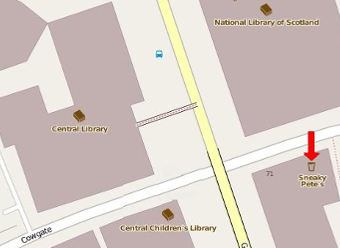
\includegraphics[width=8.5cm]{figures/with-zoom.jpg}\\[0pt]
\caption{Mapa con nivel de zoom m\'as detallado}
\label{fig-with-zoom}
\end{center}
\end{figure}

%The underlying models for these two maps are different but not unrelated. The map with 2X zoom contains fewer objects but may include more properties due to the added level of detail. The  referring expression for the target in the 1X map may or may not be the same as in the 2X map. For instance, the referring expression  ``the pub at Cowgate'' is underspecified on the 1X map, but it is minimally distinguishing on the 2X map. Changes of this kind are common in interactive applications.  The context of reference during an interaction changes in structure, in the number of objects and referable properties. The challenge for GER algorithms would be to produced an appropriate description for the modified context without starting from scratch. GER algorithms based on local (rather than global) context partitioning (e.g.,~\cite{areces08}) seem to have an advantage in this respect, and in this sense we hope that the Zoom data will help the research in the field to move forward.

 Los modelos subyacentes de estos dos mapas son diferentes, pero no sin relaci\'on. El mapa con zoom 2X contiene menos objetos, pero pueden ser m\'as propiedades debido al mayor nivel de detalle. La ER para el target en el mapa 1X puede o no puede ser la misma que en el mapa 2X. Por ejemplo, la expresi\'on referencial ``el pub en Cowgate'' es subespecificada en el mapa 1X, pero es minimal en el mapa 2X. Cambios de este tipo son comunes en aplicaciones interactivas. El contexto de referencia durante una interacci\'on, cambios en la estructura, en el n\'umero de objetos y propiedades a las cuales referirse. El desaf\'{i}o para los algoritmos GER ser\'{i}a producir una descripci\'on apropiada para el contexto modificado sin empezar desde cero. GER algoritmos basados en particiones de  contexto locales (no totales) (por ejemplo,~\cite{areces08}) parecen tener una ventaja en este sentido, y en este sentido esperamos que los datos de ZOOM ayudar\'an a que la investigaci\'on progrese.


%%%%%%%%%%%%%%%%%%%%%%%%%%%%%%%%%%%%%%%%%%%%%%%%%%%%%%%%%%%%%%%%%%%%%%%%%%%%%%%%%%%%%%%%%%%%%%%%%%%%%%%%%%%%%%%%%%%%%%%%%%%%%%%%%%%%%%%%%%%%%%%%%%%%%%%%%%
\section{Evaluaci\'on}
%%%%%%%%%%%%%%%%%%%%%%%%%%%%%%%%%%%%%%%%%%%%%%%%%%%%%%%%%%%%%%%%%%%%%%%%%%%%%%%%%%%%%%%%%%%%%%%%%%%%%%%%%%%%%%%%%%%%%%%%%%%%%%%%%%%%%%%%%%%%%%%%%%%%%%%%%%
\label{corpus-evaluacion}
%\textcolor{blue}{decidir si esta parte la dejo o no, mas me gustaria poner evaluacion para la parte en espanol}

%In this section we illustrate the use of the Zoom corpus as training and test data for a machine learning approach to GER adapted from \cite{thiago-svm}. The  goal of this evaluation is to provide reference results for future comparison with purpose-built GER algorithms, and not to present a complete GER solution for this or other domains.

%................................
\subsection{Modelo Computacional }
%................................

%The present model consists of 12 binary classifiers representing whether individual referential attributes should be selected for inclusion in an output description. The classifiers correspond to atomic attributes of the target and first landmark object ({\em type}, {\em name} and {\em others}), and relations. Referential attributes of other landmark objects were not modelled due to data sparsity and also to reduce computational costs. For similar reasons, the multivalue {\em between} relation is also presently disregarded, and `corner' relations involving two landmarks (e.g., two streets) will be modelled as two separate classification tasks.

%Two learning features were considered by each classifier:{\em landmarkCount}, which represents the number of landmark objects near the main target, and {\em DistractorCount}, which represents the number of objects of the same type as the target within the relevant context in the map.

%From the outcome of the 12 binary classifiers, a description is built by considering atomic target attributes in the first place. For every positive prediction, the corresponding atomic attribute is selected for inclusion in the output description. Next, relations are considered. If no relation is predicted, the algorithm terminates by returning an atomic description  of the main target object. If the description includes a relation, the related landmark object is selected  as well, and the algorithm is called recursively to describe the next object.

%Since every attribute that corresponds to a positive prediction is always selected, the algorithm does not regard uniqueness as a stop condition. As a result, the output description may convey a certain amount of overspecification.


El presente modelo se compone de 12 clasificadores binarios que representan si los atributos referenciales individuales deben ser seleccionados para su inclusi\'on en una descripci\'on de salida. Los clasificadores se corresponden con atributos at\'omicos del destino y objeto primer hito ({\em tipo}, {\em nombre } y {\em otros}), y las relaciones. Atributos referenciales de otros objetos emblem\'aticos no se modelaron debido a la escasez de datos y tambi\'en para reducir los costos computacionales. Por razones similares, el valor m\'ultiple {\em entre} relaci\'on es tambi\'en actualmente caso omiso, y `relaciones esquina 'que implican a dos puntos de referencia (por ejemplo, dos calles) se modelan como dos tareas de clasificaci\'on independientes.

Dos caracter\'{i}sticas de aprendizaje fueron considerados por cada clasificador:{\em landmarkCount}, que representa el n\'umero de objetos se\~nal cerca de la diana principal, y {\em DistractorCount}, que representa el n\'umero de objetos del mismo tipo que el objetivo dentro de la pertinente contexto en el mapa.

A partir de los resultados de los 12 clasificadores binarios, una descripci\'on se construye teniendo en cuenta los atributos de destino at\'omicas en el primer lugar. Por cada predicci\'on positiva, se selecciona el atributo at\'omica correspondiente para su inclusi\'on en la descripci\'on de salida. A continuaci\'on, se consideran las relaciones. Si se prev\'e ninguna relaci\'on, el algoritmo termina devolviendo una descripci\'on at\'omica del objeto target. Si la descripci\'on incluye una relaci\'on, se selecciona el objeto de punto de inter\'es relacionadas, as\'{i}, y el algoritmo se llama de forma recursiva para describir el siguiente objeto.

Puesto que cada atributo que corresponde a una predicci\'on positiva est\'a siempre seleccionado, el algoritmo no considera singularidad como una condici\'on de parada. Como resultado, la descripci\'on de salida puede transmitir una cierta cantidad de sobrevaloraci\'on.

%......................
\subsection{Procedimiento}
%......................

%We used a subset of singular descriptions from the Portuguese portion of the corpus. This comprises  821 descriptions produced in 9 scenes. Evaluation was carried out by comparing the corpus description with the system output to measure overall accuracy (i.e., the number of exact matches between the two descriptions), Dice \cite{dice} and MASI \cite{masi} coefficients (i.e., the degree of overlap between the algorithm output and the corresponding corpus description).

%Following \cite{thiago-svm}, we built a GER model using support vector machines with radial basis function kernel. The classifiers were trained and tested using 6-fold cross validation. Optimal parameters were selected using grid search as follows:for each step in the main cross-fold validation, one fold is reserved for testing, and the remaining $k-1$ folders are subject  to a second cross-validation procedure in which different parameter combinations are attempted. The $C$ parameter is assigned the values 1, 10, 100 and 1000, and $\gamma$ is assigned 1, 0.1, 0.001 and 0.0001. The best-performing parameter set is selected to build a classifier trained from the $k-1$ folders, and tested on the test data. This procedure is repeated for every iteration of the main cross-validation procedure.

Se utiliz\'o un subconjunto de descripciones singulares de la parte portuguesa del corpus. Esto comprende 821 descripciones producidos en 9 escenas. La evaluaci\'on se llev\'o a cabo mediante la comparaci\'on de la descripci\'on corpus ante la salida del sistema para medir la precisi\'on global (es decir, el n\'umero de coincidencias exactas entre las dos descripciones), dados \cite{dice} y MASI \cite{masi} coeficientes (es decir, el grado de solapamiento entre la salida del algoritmo y la descripci\'on corpus correspondiente).

Siguiendo \cite{thiago-svm}, construimos un modelo GER uso de m\'aquinas de vectores soporte con radial kernel de funci\'on de base. Los clasificadores se capacit\'o y sometieron a pruebas de 6 veces la validaci\'on cruzada. Los par\'ametros \'optimos fueron seleccionados mediante b\'usqueda en la red de la siguiente manera:para cada paso en el principal validaci\'on cruzada veces, un solo reba\~no est\'a reservado para las pruebas, y los restantes $k-1$ carpetas est\'an sujetas a un segundo procedimiento de validaci\'on cruzada en la que diferentes par\'ametros combinaciones se intentan. El par\'ametro $C$ se le asignan los valores de 1, 10, 100 y 1000, y $\gamma$ es asignado en 1, 0,1, 0,001 y 0,0001. El conjunto de par\'ametros de mejor desempe\~no es seleccionada para construir un clasificador entrenado desde las carpetas $k-1$, y probado en los datos de prueba. Este procedimiento se repite para cada iteraci\'on del procedimiento principal de validaci\'on cruzada.
%......................
\subsection{Resultados de GER }
%......................

%Table \ref{tab-reg-results} summarizes the results obtained by the GER algorithm built from SVM classifiers, those obtained by a baseline system representing a relational extension of the Dale \& Reiter Incremental Algorithm, and by a Random selection strategy.  
Tabla \ref{tab-reg-results} resume los resultados obtenidos por el algoritmo GER construido a partir de SVM clasificadores, los obtenidos mediante un sistema de l\'{i}nea de base que representa una extensi\'on relacional de la \& Reiter Incremental Algoritmo Dale, y por una estrategia de selecci\'on aleatoria.

% these results are for SVM.All.VAR-   compared to the AEI- baseline
\begin{table}[H]
\begin{center}
\caption{Resultados de la GER}
\label{tab-reg-results}
\begin{tabular} {  l c c c }
\hline
{Algorithm}							& {Acc.} 	& { Dice}		& MASI \\ \hline 
SVM											& 0.15		& 0.51			& 0.28 \\
Incremental							& 0.04		& 0.53			& 0.21 \\
Random selection       	& 0.03    & 0.45      & 0.15 \\
\hline
\end{tabular}
\end{center}
\end{table}

%In what follows we compare accuracy scores obtained by every algorithm pair using the chi-square test, and we compare {\em Dice} scores using {\em Wilcoxon's} signed-rank test.

%In terms of overall accuracy\footnote{And also in terms of MASI scores, although this is presently not further discussed.}, the SVM approach outperforms both alternatives. The difference from the second best-performing algorithm (i.e., the Incremental approach) is highly significant ($\chi^{2}=$ 79.87, df=1, p$<$0.0001). Only in terms of Dice scores an opposite effect is observed (T=137570.5, p$=$ 0.01413). 

%We also assessed the performance of the individual classifiers. Table \ref{tab-svm-results} shows these results as measured by precision (P), recall (R), F1-measure (F1) and area under the ROC curve (AUC). 


En lo que sigue se comparan precisi\'on resultados obtenidos por cada par algoritmo mediante la prueba de chi cuadrado, y comparamos {\em dados} puntajes utilizando la prueba de rangos con signo {\em de Wilcoxon}.

En t\'erminos de precisi\'on global \footnote{Y tambi\'en en cuanto a las puntuaciones MASI, aunque actualmente no se discute m\'as.}, El m\'etodo SVM supera a ambas alternativas. La diferencia con el segundo algoritmo de mejor rendimiento (es decir, el enfoque incremental) es altamente significativo ($\chi^{2}=$ 79,87, df = 1, p$<$ 0,0001). S\'olo en cuanto a las puntuaciones de dice se observa el efecto contrario (T = 137570.5, p$=$0,01413).

Tambi\'en se evalu\'o el desempe\~no de los clasificadores individuales. Tabla \ref{tab-svm-results} muestra estos resultados, medida por la precisi\'on (P), memoria (R), F1-medida (F1) y el \'area bajo la curva ROC (AUC).

%these are the rsults for the training over the set of ALL speakers 
\begin{table}[H]
\begin{center}
\footnotesize{
\caption{Resultados del clasificador}
\begin{tabular}{l c c c c }
\hline
{{Classifier}}	& {P} & {R} & {$F_{1}$} & {AUC} \\
\hline
{{tg\_type}} 			& 0.95 & 1.00 & 0.98 & 0.25 \\
{{tg\_name}}			& 0.09 & 0.05 & 0.07 & 0.41 \\
{{tg\_other}}			& 0.00 & 0.00 & 0.00 & 0.05 \\                               
{{lm\_type}}			& 0.93 & 1.00 & 0.96 & 0.44 \\                               
{{lm\_name}}			& 0.97 & 1.00 & 0.98 & 0.35 \\                               
{{lm\_other}}			& 0.00 & 0.00 & 0.00 & 0.43 \\                               
{{next-to}}				& 0.50 & 0.24 & 0.32 & 0.63 \\                               
{{right-of}}			& 0.00 & 0.00 & 0.00 & 0.28 \\                               
{{left-of}}				& 0.00 & 0.00 & 0.00 & 0.27 \\                               
{{in-front-of}}		& 0.00 & 0.00 & 0.00 & 0.42 \\                               
{{behind-of}}			& 0.00 & 0.00 & 0.00 & 0.17 \\                               
{{in/on/at}} 			& 0.60 & 0.60 & 0.60 & 0.61 \\                               
\hline                   
\end{tabular}
\label{tab-svm-results}
}
\end{center}
\end{table}
\normalsize

%From these results we notice that highly frequent attributes (e.g., type and name) were classified  with high accuracy, whereas others (e.g., multivalue attributes and relations) were not. 

A partir de estos resultados nos damos cuenta de que los atributos muy frecuentes (por ejemplo, el tipo y nombre) se clasificaron con gran precisi\'on, mientras que otros (por ejemplo, los atributos de varios valores y relaciones) no lo eran.

%%%%%%%%%%%%%%%%%%%%%%%%%%%%%%%%%%%%%%%%%%%%%%%%%%%%%%%%%%%%%%%%%%%%%%%%%%%%%%%%%%%%%%%%%%%%%%%%%%%%%%%%%%%%%%%%%%%%%%%%%%%%%%%%%%%%%%%%%%%%%%%%%%%%%%%%%%	       >2






\section{Caso de estudio del ZOOM corpus}
\label{sec:caso_estudio}

En esta secci\'on presentamos tres casos de estudio particulares, de generaci\'on autom\'atica de ER para mapas del ZOOM corpus. Dividimos el estudio en 3 partes, en la Secci\'on \ref{sec:sinzoom} veremos un mapa sin zoom el cual se muestra en la Figura \ref{mapa-zoom} y cuyo target es singular. En la Secci\'on \ref{sec:conzoom} analizaremos la GER con el mismo target pero ahora con zoom 2X, el mapa usado se muestra en la Figura \ref{mapa-zoom2x}. En la Secci\'on \ref{sec:plural} veremos el mismo mapa de la Secci\'on \ref{sec:sinzoom} pero con target plural, es decir con 2 targets, el mapa se muestra en Figura \ref{mapa-zoom-plural}.

%  Veremos las diferencias entre esos mapas a nivel de informaci\'on disponible, obtendremos a partir de cada imagen el modelo subyacente que usar\'a el algoritmo y a partir de las ER's del corpus obtendremos las probabilidades de uso de las palabras, para luego ejecutar el algoritmo. Compararemos las ER's dadas por el algoritmo con las que dieron las personas.

%En cada uno de los mapas, el o los targets est\'an se\~nalados por flechas rojas, seg\'un la leyenda que se ubica a la derecha, podemos decir que si se trata de una iglesia, o restaurantes, etc. 
%
%\textcolor{blue}{
%Podria explicar un poco porque restringimos el modelo... a parte de lo que se ve en el mapa. paper Incremental generation of spacial referring expressions in situated dialog cuenta un poco como generar las ER de un robot en tiempo real, van acotando el entorno. Tambien hablan de las preferencias pero ponen nombres raros topologial constrstivem topological relative topological proyective contrastive proyective relative. (Bryant et al. 1992 Gapp 1995) above/below sobre in front of/behind y de esta sobre to the right of / to the left of
%}


\subsection{Singular sin zoom}
\label{sec:sinzoom}


En la Tabla \ref{freq-mapa} se muestran las 10 expresiones referenciales m\'as frecuentes generadas por las personas que participaron 
en la recolecci\'on del corpus para el mapa de la Figura \ref{mapa-zoom}. Se indica la cantidad de veces que aparecieron en el corpus, 
que equivale al n\'umero de distintas personas que independientemente decidieron usar la misma ER para referirse al target. 
Tambi\'en se indica sin son subespecificadas (SubE) o sobreespecificadas (SobreE). Notar que las que no son 
ni subespecificadas, ni sobreespecificadas, son minimales.


%\end{figure}
\begin{figure}
\centering
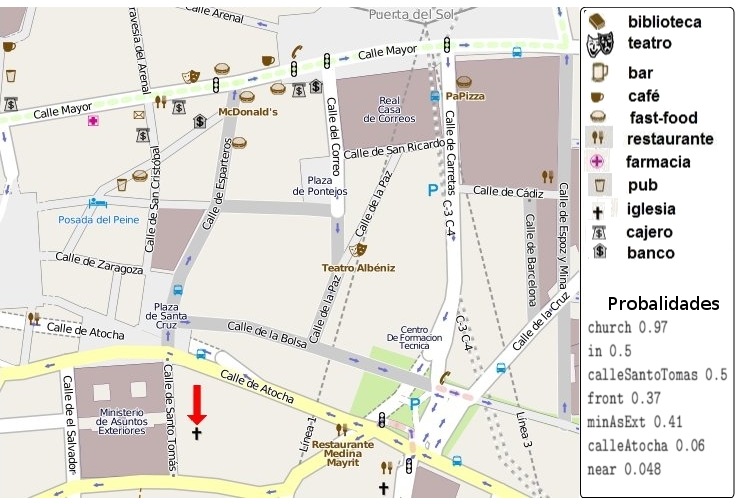
\includegraphics[width=\textwidth]{images/corpus/mapa6-prob.png}\\[0pt]
\caption{Imagen del ZOOM corpus con target singular}
\label{mapa-zoom}
\end{figure}


%\DeclareFloatFont{tiny}{\tiny}% "scriptsize" is defined by floatrow, "tiny" not

\begin{table}[H]
{\footnotesize
%\texttiny
%\floatsetup[table]{font=tiny}
\begin{center}
\begin{tabular}{|l|l|c|c|c|c|}
\hline
&ER 					      & \# &  \% & SubE & SobreE\\ \hline \hline
1&La iglesia 																																		 &16&19.7\%  & X & \\ \hline
2&Iglesia en la calle de Santo Tom\'as																									 &15&18.5\% 	&  & \\ \hline
3&Iglesia en la calle de Santo Tom\'as frente al Ministerio de Asuntos Exteriores        &11&13.6\% &  &X \\ \hline
%&Asuntos Exteriores& &&&\\ \hline
4&Iglesia frente al Ministerio de Asuntos Exteriores 													 &11&13\% &  & \\ \hline
5&Iglesia en la calle Santo Tom\'as cerca del Ministerio de Asuntos Exteriores        &2 &2.5\% &  &X \\ \hline
%&Asuntos Exteriores& & & & \\ \hline
6&Iglesia en la calle de Atocha																									 &2&2.5\%  &  & \\ \hline
7&En calle de Santo Tom\'as 																													 &2&2.5\% 	& X & \\ \hline
8&Iglesia que est\'a en la Calle de Santo Tom\'as y Atocha, frente al 									 &2&2.5\%	&  &X \\ 
&Ministerio de Asuntos Exteriores																		 &&&& \\ \hline
9&Iglesia que est\'a en la Calle de Santo Tom\'as y Atocha										 &2&2.5\% 	&  &X \\ \hline
10&Iglesia cerca del Ministerio de Asuntos Exteriores														 &1&1.2\% 	&  & \\ \hline
\end{tabular}
\caption{10 ER m\'as frecuentes del corpus para el mapa de la Figura \ref{mapa-zoom}.}\label{freq-mapa}
\end{center}
}%\end{tiny}
\end{table}


Para ejecutar el algoritmo necesitamos definir el vocabulario del modelo, es decir las palabras que vamos a usar al correr el algoritmo, la sem\'antica del mismo. Estas palabras fueron sacadas de la anotaci\'on del corpus, el cual est\'a anotado en ingl\'es. 

%Algunas personas dijeron ``en la esquina de...'', eso fue anotado como ``between'' y luego 2 calles, esta palabra no fue usada para correr el algoritmo porque tiene 2 par\'ametros, en cambio usamos ``in'' para ambas calles, con esa modificaci\'on, no estamos perdiendo informaci\'on ya que si el algoritmo da ambas calles, lo podr\'iamos realizar como ``esquina''. Se muestra el vocabulario y las probabilidades de uso de las palabras del vocabulario, sacadas del corpus, para el mapa de la Figura \ref{mapa-zoom}.
Para calcular las probabilidades de uso se tuvieron en cuenta las ER que dieron las personas, incluso las que eran subespecificadas, pero no las que no eran ciertas, un total de 63 ER fueron las que cumpl\'ian con esas condiciones. Se cont\'o la cantidad de veces que aparec\'ia la palabra, teniendo en cuenta que si aparec\'ia 2 veces en la misma ER se contaba s\'olo 1 vez, a fin de tener siempre probabilidades entre 0 y 1, y luego se dividi\'o sobre 63 que fueron la cantidad de ER que eran v\'alidas.

\begin{table}[H]
\begin{small}
\begin{center}
\begin{tabular}{|l|c|}
\hline
Palabra 					      &  Probabilidad\\ \hline \hline

church & 0.968\\
in & 0.5079\\
in-front-of & 0.365\\
near & 0.0476\\
ministerioAsuntosExteriores & 0.41\\
calleDeSantoTomas & 0.5079\\
calleDeAtocha & 0.06\\
\hline
\end{tabular}
\caption{Probabilidad de las palabras del dominio.}\label{prob-vocabulario}
\end{center}
\end{small}
\end{table}
%\begin{table}[H]
%\begin{small}
%\begin{center}
%\begin{tabular}{|l|}
%\hline
%Palabra 					     Probabilidad\\ \hline \hline
%
%church  0.968\\
%in 0.5079\\
%in-front-of 0.365\\
%near 0.0476\\
%MinAsExt  0.41\\
%CalleSantoTomas 0.5079\\
%CalleAtocha 0.06\\
%\hline
%\end{tabular}
%\caption{Probabilidad de las palabras del dominio.}\label{prob-vocabulario}
%\end{center}
%\end{small}
%\end{table}

El modelo que representa el fragmento del mapa de la Figura \ref{mapa-zoom}, al sur de la Calle de Atocha, se muestra en la Figura \ref{modelo-mapa-zoom}

\begin{figure}[ht]
\centering
\begin{tikzpicture}
  [
    n/.style={circle,draw,inner sep=5pt,node distance=4cm},
    aArrow/.style={scale=10,->, >=stealth, thick,
    shorten <= 1pt, shorten >= 1pt},
  ]
	\node[n,label=below:{
    \relsize{-2}$\begin{array}{c}
     \nStreet\end{array}$}] (a) {$str17$};		
			
	\node[n,label=below:{
    \relsize{-2}$\begin{array}{c}
      \nStreet\\[-3pt] 
      \nCalleDeElSalvador\end{array}$}, right of=a] (b) {$str12$};
  
	\node[n,label=below:{
    \relsize{-2}$\begin{array}{c}
      \nStreet\\[-3pt] 
      \nCalleDeLaCruz\end{array}$}, right of=b] (m) {$str16$};		 

\node[n,label=above:{
    \relsize{-2}$\begin{array}{c}
      \nStreet\\[-3pt] 
      \nCalleSantoTomas\end{array}$}, above of=b] (c) {$str10$};	
				
 \node[n,label=above:{
    \relsize{-2}$\begin{array}{c}
      \nBuilding\\[-3pt] 
      \nMinAsExt\end{array}$}, above of=a] (f) {$min1$};	
					
  \node[n,label=below:{
    \relsize{-2}$\begin{array}{c}
     \nChurch\end{array}$}, above of=f] (g) {$church1$};
			
 \node[n,label=below:{
    \relsize{-2}$\begin{array}{c}
     \nChurch\end{array}$}, right of=c] (d) {$church2$};
			
  \node[n,label=above:{
    \relsize{-2}$\begin{array}{c}
      \nRestaurante\\[-3pt] 
      MedinaMayrit\end{array}$}, above of=d] (h) {$rest3$};			
			
 \node[n,label=above:{
    \relsize{-2}$\begin{array}{c}
      \nStreet\\[-3pt] 
      \nCalleAtocha\end{array}$}, above of=c] (e) {$str9$};		

\node[n,label=below:{
    \relsize{-2}$\begin{array}{c}
      \nRestaurante\end{array}$}, right of=m] (k) {$rest4$};

\node[n,label=below:{
    \relsize{-2}}, right of=d] (i) {$d$};
		
 \node[n,label=above:{
    \relsize{-2}$\begin{array}{c}
      \nStreet\\[-3pt] 
      \nCalleDeCarretas\end{array}$}, above of=i] (j) {$str15$};	

%\node[n,label=below:$str17\nStreet$,label=above:{
 %   \relsize{-2}}, below of=k] (n) {};				
 \draw [aArrow,<->,bend right=40] (g) to node[auto,swap]{\relsize{-3}$\nFrenteCerca$} (f);
% \draw [aArrow,bend right=40] (f) to node[auto,swap]{\relsize{-3}$\nFrenteCerca$} (g);

 \draw [aArrow,bend right=40] (g) to node[auto,swap]{\relsize{-3}$\nIn$} (c);
 \draw [aArrow,bend right=20] (g) to node[auto,swap]{\relsize{-3}$\nIn$} (e);

 \draw [aArrow,bend right=40] (d) to node[auto,swap]{\relsize{-3}$\nIn$} (m);
 \draw [aArrow,<->,bend right=-10] (d) to node[auto,swap]{\relsize{-3}$\nFrenteCerca$} (i);
 %\draw [aArrow,bend right=40] (i) to node[auto,swap]{\relsize{-3}$\nFrente$} (d);
 \draw [aArrow,<->,bend right=40] (k) to node[auto,swap]{\relsize{-3}$\nCerca$} (d);
 %\draw [aArrow,bend right=40] (d) to node[auto,swap]{\relsize{-3}$\nCerca$} (k);
 \draw [aArrow,<->,bend right=80] (k) to node[auto,swap]{\relsize{-3}$\nCerca$} (h);

 \draw [aArrow,bend right=40] (k) to node[auto,swap]{\relsize{-3}$\nIn$} (m);
 \draw [aArrow,<->,bend right=20] (k) to node[auto,swap]{\relsize{-3}$\nFrenteCerca$} (i);
% \draw [aArrow,bend right=40] (i) to node[auto,swap]{\relsize{-3}$\nFrente$} (k);
 \draw [aArrow,bend right=20] (h) to node[auto,swap]{\relsize{-3}$\nIn$} (e);
 \draw [aArrow,bend right=-20] (h) to node[auto,swap]{\relsize{-3}$\nIn$} (j);

 \draw [aArrow,bend right=30] (f) to node[auto,swap]{\relsize{-3}$\nIn$} (c);
 \draw [aArrow,bend right=40] (f) to node[auto,swap]{\relsize{-3}$\nIn$} (e);
 \draw [aArrow,bend right=40] (f) to node[auto,swap]{\relsize{-3}$\nIn$} (a);
 \draw [aArrow,bend right=40] (f) to node[auto,swap]{\relsize{-3}$\nIn$} (b); 

 \draw [aArrow,bend right=5] (i) to node[auto,swap]{\relsize{-3}$\nIn$} (e);
 \draw [aArrow,bend right=40] (i) to node[auto,swap]{\relsize{-3}$\nIn$} (m);
%\draw[dotted] (-0.5,-1.1) rectangle (10.5,3.1);

 \end{tikzpicture}
\caption{Grafo del contexto de la Figura \ref{mapa-zoom}}
\label{modelo-mapa-zoom}
\end{figure}

Se ejecut\'o el algoritmo 1000 veces, las 10 f\'ormulas m\'as frecuentes, y la frecuencia dada por el algoritmo fueron las que se muestran en la Tabla \ref{freq-mapa-algoritmo}


\begin{tabular}{|l|l|c|c|}
\hline
 &Posible realizaci\'on de la ER &  \# & \% \\ \hline
1&Iglesia en la calle de Santo Tom\'as   & & \\ \hline
2&Iglesia en la calle de Santo Tom\'as frente al Ministerio de Asuntos Exteriores        & &13.6\%  \\ \hline
%&Asuntos Exteriores& &&&\\ \hline
3&Iglesia frente al Ministerio de Asuntos Exteriores                                   & & \\ \hline                                        
4&Iglesia en la calle Santo Tom\'as cerca del Ministerio de Asuntos Exteriores        & &2.5\%  \\ \hline
%&Asuntos Exteriores& & & & \\ \hline
5&Iglesia en la calle de Atocha                                                       & & \\ \hline                                           
6&En calle de Santo Tom\'as                                                                        & & \\ \hline                                
7&Iglesia que est\'a en la Calle de Santo Tom\'as y Atocha,                                       & &\% \\ \hline
&frente al Ministerio de Asuntos Exteriores                                         && \\ \hline                                            
8&Iglesia que est\'a en la Calle de Santo Tom\'as y Atocha                           & & \\ \hline
9&Iglesia cerca del Ministerio de Asuntos Exteriores                                 & & \\ \hline                                              
\end{tabular}
\caption{10 ER m\'as frecuentes dadas por el algoritmo para el grafo de la Figura \ref{modelo-mapa-zoom}.}\label{freq-mapa-algoritmo}
\end{center}
}%\end{tiny}
\end{table}


\begin{enumerate}
\item Ex-iglesia.(T) \& Ex-in.(Ex-CalleDeSantoTomas.(T))->234
\item Ex-frente.(Ex-MinisterioAsuntosExteriores.(T))->202
\item Ex-iglesia.(T) \& Ex-in.(Ex-CalleDeAtocha.(T))->87
\item Ex-cerca.(Ex-MinisterioAsuntosExteriores.(T))->79
\item Ex-frente.(Ex-frente.(Ex-iglesia.(T))) \& Ex-in.(Ex-CalleDeSantoTomas.(T)): church1->74
\end{enumerate}

La f\'ormula (1) ``Ex-iglesia.(T) \& Ex-in.(Ex-CalleDeSantoTomas.(T))'' se podr\'ia realizar como ``La iglesia que est\'a en la Calle De Santo Tom\'as''. La f\'ormula (2) se podr\'ia realizar como ``La que est\'a al frente del Ministerio de Asuntos Exteriores''. La f\'ormula (3) como ``La iglesia de la Calle De Atocha''. La f\'ormula (4) con ``Una que esta cerca del Ministerio de Asuntos Exteriores'' y la (5) ``La que esta en Calle de Santo Tomas al frente de algo que tiene al frente una iglesia''. Este \'ultimo tipo de f\'ormulas son las menos deseadas y las menos naturales, podemos ver que en este caso la di\'o el 7\% de las veces, lo cual no es muy alto. Todas las f\'ormulas que di\'o el algoritmo en 1000 ejecusiones con sus respectivas frecuencias se muestran en el Ap\'endice en Secci\'on \ref{er-mapa-zoom}.


\begin{table}[H]
{\footnotesize
\begin{center}
\begin{tabular}{|l|c|c|}
\hline
ER 					      &  Frecuencia & Frecuencia-Alg\\ \hline \hline
La iglesia 																																		 &0.197\%  &  -\\ \hline
Iglesia en calle Santo Tomas																									 &0.185\% 	& 0.197\%  \\ \hline
Iglesia en calle Santo Tomas frente al Ministerio de Asuntos Exteriores        &0.1358\% & 0.001\% \\ \hline
Iglesia  frente al Ministerio de Asuntos Exteriores 													 &0.1358\% & 0.071\%  \\ \hline
Iglesia en calle Santo Tomas cerca del Ministerio de Asuntos Exteriores        &0.0246\% & 0.00\%  \\ \hline
La Iglesia en Calle de Atocha																									 &0.0246\%  &0.087\%  \\ \hline
Calle de santo tomas 																													 &0.0246\% 	& -  \\ \hline
La iglesia que est\'a en la Calle de Santo Tom\'as y Atocha, 									 &0.0246\%	& 0.00\% \\ 
frente al Ministerio de Asuntos Exteriores																		 && \\ \hline
La iglesia que est\'a en la Calle de Santo Tom\'as y Atocha										 &0.0246\% 	& 0.00\%  \\ \hline
Iglesia cerca del Ministerio de Asuntos Exteriores														 &0.0123\% 	& 0.004\%  \\ \hline
NO-ERA-ER																																			 &0.222\%  &\\ \hline \hline
Totales& &\\
\hline
\end{tabular}
\caption{Comparaci\'on ER del corpus y las dadas por el algoritmo.}\label{compara-corpus-alg}
\end{center}
}
\end{table}

Notar que las personas dieron 10 tipos de ER, de los cuales 2 son subespecificadas, al ser subespecificadas, el algoritmo no las gener\'o, son las que est\'an marcadas en la Tabla \ref{compara-corpus-alg} con '-'. La segunda m\'as frecuente dada por las personas, que en realidad fue la primer ER m\'as frecuente, tambi\'en fue la m\'as frecuente dada por el algoritmo. Consideramos que el algoritmo no gener\'o las ER ``La iglesia que est\'a en la Calle de Santo Tom\'as y Atocha, frente al Ministerio de Asuntos Exteriores'' y ``La iglesia que est\'a en la Calle de Santo Tom\'as y Atocha'' por tener CalleDeAtocha una probabilidad de uso muy baja 0.06.



\subsection{Singular con zoom 2x}
\label{sec:conzoom}
En la Figura \ref{mapa-zoom2x} se ve el nombre de la iglesia, ``Parroquia de Santa Cruz'', lo cual no se ve en la Figura \ref{mapa-zoom}, otra cosa que se puede ver en el mapa con zoom2x es el nombre de la calle que esta abajo ``Calle de la Concepci\'on Jeronima'', en este mapa no se puede ver el nombre del Ministerio de Asuntos Exteriores, por lo tanto lo \'unico que se ve en la Calle de Santo Tom\'as es la iglesia target. 

 En la Tabla \ref{freq-mapa-zoom2x} se muestran las ER, la cantidad de ocurrencia en el corpus

\begin{figure}
\centering
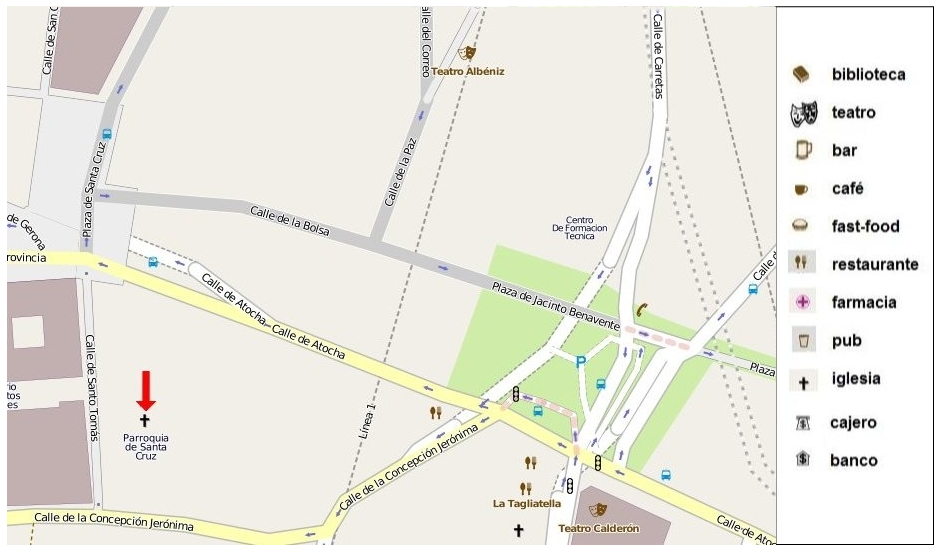
\includegraphics[width=\textwidth]{images/corpus/mapa16.png}\\[0pt]
\caption{Imagen con zoom 2X, target singular}
\label{mapa-zoom2x}
\end{figure}

\begin{table}[H]
{\footnotesize
\begin{center}
\begin{tabular}{|l|c|c|c|c|}
\hline
ER 					      & Cantidad &  Frecuencia & SubE&SobreE \\ \hline \hline
Parroquia de Santa Cruz        												 &		44&	\%  & NO &NO \\ \hline
Parroquia de Santa Cruz en Calle De Santo Tomas        &	 9  &	\%	& NO&SI\\ \hline
Parroquia de Santa Cruz en Calle De Santo Tomas        &	 3  &	\%	& NO&SI\\
entre Calle De Atocha y De La Concepci\'on Jer\'onima  &	    &			&  &\\  \hline
Calle De Santo Tomas	        												 &		1 &	\%	&SI&NO\\  \hline
Iglesia de la Parroquia de Santa Cruz	      					 &		2 &	\%	&NO&SI\\  \hline
Parroquia de Santa Cruz en Calle De Santo Tomas  			 &	  3 &	\%	&NO&SI\\  
cerca de Ministerio de Asuntos Exteriores							 &	  &		& &\\  \hline
Parroquia de Santa Cruz en Calle De Santo Tomas y      &	 4 &	\%	& NO&SI\\  
De La Concepci\'on Jer\'onima  												 &	  &					& &\\  \hline
Iglesia de la Parroquia de Santa Cruz	en       &		2&	\%	&NO&SI\\  
Calle De Santo Tomas													 				 &		 &	    &  & \\ \hline
Iglesia cerca deL Ministerio de Asuntos Exteriores				&	 1 &		&NO&SI\\  \hline
Parroquia de Santa Cruz  &	  1&	\%	&NO&SI\\  
cerca de Ministerio de Asuntos Exteriores				&	  &		&&\\  \hline
Parroquia de Santa Cruz en Calle De Atocha  &	  1&	\%	&NO&SI\\  
cerca de Ministerio de Asuntos Exteriores				&	  &		&&\\  \hline
Iglesia				&  1 &	\%	&SI&NO\\  \hline
NO ERA ER				&	8  &	\%	& &\\  \hline
\hline
\hline
Totales	&81	&	100\% &	3 minimales &\\
\hline
\end{tabular}
\caption{ER del corpus dadas por humanos para el mapa de la Figura \ref{mapa-zoom2x}.}\label{freq-mapa-zoom2x}
\end{center}
}
\end{table}

El vocabulario y las probabilidades de uso sacadas del corpus, para el mapa de la Figura \ref{mapa-zoom2x} es el siguiente:

ParroquiaDeSantaCruz 66/73=0.904\\
in 23/73=0.315\\
CalleSantoTomas 22/73=0.301\\
CalleDeAtocha 4/73=0.055\\
CalleDeLaConcepcionJeronima 7/73=0.096\\
iglesia 6/73=0.082\\
cerca 6/73=0.082\\
MinisterioDeRelacionesExteriores 5/73=0.068 


Y el modelo en el cual vamos a notar muchas diferencias con respecto al modelo de la Figura \ref{mapa-zoom} y esto se debe a que al acercar el zoom del mapa, se ven m\'as detalladamente algunas cosas, por ejemplo se ve que la Iglesia no est\'a en la Calle De Atocha como parec\'ia en el mapa mostrado en la Figura \ref{mapa-zoom}. Se agrega la Calle De La Concepci\'on Jer\'onima que no se ve\'ia en el mapa anterior. Notar que no se ve el nombre del Ministerio de Asuntos Exteriores. Se agrega el nombre ``Parroquia de Santa Cruz'' que no se ve\'ia en el otro mapa. Aparece una nueva calle la que esta en la parte superior de la manzana de la iglesia, de la cual no sabemos el nombre, el identificador ser\'a str25. Aparece el nombre de la calle (Calle de Carretas, cuyo identificar es str15) en la que esta el restaurant Medina Mayrit, pero desaparece el nombre del mismo. El building con identificar d, en este mapa se ve que es un teatro, el Teatro Calderón, tambi\'en aparece en el mapa el restaurante ``La Tagliatela'' al lado de un restaurante sin nombre, uno de esos restaurantes se pod\'a ver en el mapa sin zoom. Vamos a suponer que el que se pod\'ia ver en el mapa sin zoom era ``La Tagliatela'' a fin de conservar los mismos identificadores. Notar que dejamos de ver el nombre de la calle en la cual se ubica el teatro y los restaurantes reci\'en nombrados.

\begin{figure}[ht]
\centering
\begin{tikzpicture}
  [
    n/.style={circle,fill,draw,inner sep=3pt,node distance=4cm},
    aArrow/.style={->, >=stealth, thick, shorten <= 1pt, shorten >= 1pt},	
  ]
	\node[n,label=left:$str17$,label=below:{
    \relsize{-2}$\begin{array}{c}
     \nStreet\end{array}$}] (a) {};		
	 \node[n,label=left:$min1$,label=above:{
    \relsize{-2}$\begin{array}{c}
      \nBuilding\end{array}$}, above of=a] (f) {};	
					 
	\node[n,label=left:$church1$,label=above:{
    \relsize{-2}$\begin{array}{c}
		 \nChurch\\[-3pt] 
     \nParroquiaDeSantaCruz\end{array}$}, above of=f] (g) {};
	\node[n,label=right:$str22$,label=above:{
    \relsize{-2}$\begin{array}{c}
      \nStreet\\[-3pt] 
      \nCalleDeLaConcepcionJeronima\end{array}$}, above of=g] (z) {};
			
	\node[n,label=right:$str25$,label=above:{
    \relsize{-2}$\begin{array}{c}
      \nStreet\end{array}$}, right of=z] (y) {};	
				
	\node[n,label=above:$str12$,label=below:{
    \relsize{-2}$\begin{array}{c}
      \nStreet\\[-3pt] 
      \nCalleDeElSalvador\end{array}$}, right of=a] (b) {};
   
	\node[n,label=left:$str16$,label=below:{
    \relsize{-2}$\begin{array}{c}
      \nStreet\end{array}$}, right of=b] (m) {};		 

  \node[n,label=below:$str10$,label=above:{
    \relsize{-2}$\begin{array}{c}
      \nStreet\\[-3pt] 
      \nCalleSantoTomas\end{array}$}, above of=b] (c) {};	
			
  \node[n,label=left:$church2$,label=below:{
    \relsize{-2}$\begin{array}{c}
     \nChurch\end{array}$}, right of=c] (d) {};
			
  \node[n,label=below:$rest3$,label=above:{
    \relsize{-2}$\begin{array}{c}
      \nRestaurante\end{array}$}, above of=d] (h) {};			
			
  \node[n,label=left:$str9$,label=above:{
    \relsize{-2}$\begin{array}{c}
      \nStreet\\[-3pt] 
      \nCalleAtocha\end{array}$}, above of=c] (e) {};		

  \node[n,label=left:$rest4$,label=right:{
    \relsize{-2}$\begin{array}{c}
      \nRestaurante\\[-3pt] 
      \nLaTagliatella\end{array}$}, right of=m] (k) {};

 \node[n,label=left:$rest5$,label=below:{
    \relsize{-2}$\begin{array}{c}
      \nRestaurante\end{array}$}, below of=k] (w) {};

  \node[n,label=above:$thea0$,label=below:{
    \relsize{-2}$\begin{array}{c}
      \nTeatroCalderon\end{array}$}, right of=d] (i) {};
		
  \node[n,label=right:$str15$,label=above:{
    \relsize{-2}$\begin{array}{c}
      \nStreet\\[-3pt] 
      \nCalleDeCarretas\end{array}$}, right of=h] (x) {};	

%\node[n,label=below:$str17\nStreet$,label=above:{
 %   \relsize{-2}}, below of=k] (n) {};				
 \draw [aArrow,<->,bend right=40] (g) to node[auto,swap]{\relsize{-3}$\nFrenteCerca$} (f);
% \draw [aArrow,bend right=40] (f) to node[auto,swap]{\relsize{-3}$\nFrenteCerca$} (g);

 \draw [aArrow,bend right=40] (g) to node[auto,swap]{\relsize{-3}$\nIn$} (c);
 \draw [aArrow,bend right=20] (g) to node[auto,swap]{\relsize{-3}$\nIn$} (z);
 \draw [aArrow,bend right=20] (g) to node[auto,swap]{\relsize{-3}$\nIn$} (y);
 \draw [aArrow,bend right=40] (d) to node[auto,swap]{\relsize{-3}$\nIn$} (m);
 \draw [aArrow,<->,bend right=-20] (d) to node[auto,swap]{\relsize{-3}$\nFrenteCerca$} (i);
 %\draw [aArrow,bend right=40] (i) to node[auto,swap]{\relsize{-3}$\nFrente$} (d);
 \draw [aArrow,<->,bend right=40] (k) to node[auto,swap]{\relsize{-3}$\nCerca$} (d);
 \draw [aArrow,<->,bend right=40] (k) to node[auto,swap]{\relsize{-3}$\nCerca$} (w);
 %\draw [aArrow,bend right=40] (d) to node[auto,swap]{\relsize{-3}$\nCerca$} (k);
 \draw [aArrow,<->,bend right=40] (k) to node[auto,swap]{\relsize{-3}$\nIn$} (x);
 \draw [aArrow,bend right=40] (k) to node[auto,swap]{\relsize{-3}$\nIn$} (m);
 \draw [aArrow,<->,bend right=40] (k) to node[auto,swap]{\relsize{-3}$\nFrenteCerca$} (i);
% \draw [aArrow,bend right=40] (i) to node[auto,swap]{\relsize{-3}$\nFrente$} (k);
 \draw [aArrow,bend right=20] (h) to node[auto,swap]{\relsize{-3}$\nIn$} (e);
 \draw [aArrow,bend right=20] (h) to node[auto,swap]{\relsize{-3}$\nIn$} (j);

 \draw [aArrow,bend right=30] (f) to node[auto,swap]{\relsize{-3}$\nIn$} (c);
 \draw [aArrow,bend right=40] (f) to node[auto,swap]{\relsize{-3}$\nIn$} (e);
 \draw [aArrow,bend right=40] (f) to node[auto,swap]{\relsize{-3}$\nIn$} (a);
 \draw [aArrow,bend right=40] (f) to node[auto,swap]{\relsize{-3}$\nIn$} (b); 

 \draw [aArrow,bend right=5] (i) to node[auto,swap]{\relsize{-3}$\nIn$} (e);
 \draw [aArrow,bend right=40] (i) to node[auto,swap]{\relsize{-3}$\nIn$} (m);

 \end{tikzpicture}
\caption{Grafo del contexto \ref{mapa-zoom2x}}
\label{modelo-mapa-zoom2x}
\end{figure}

Notar que en el modelo no esta el Ministerio de Asuntos Exteriores, pero la probabilidad di\'o mayor que 0, esto se debe a que como en la obtenci\'on del corpus los mapas se mostraron aleatoriamente, algunas personas vieron el mapa sin zoom antes, y recordaron que ese edificio que se v\'e en el mapa, es el Ministerio de Asuntos Exteriores, como no todas las personas lo vieron es que no podemos agregarlo al modelo.


\subsection{Plural sin zoom}
\label{sec:plural}
\begin{figure}
\centering
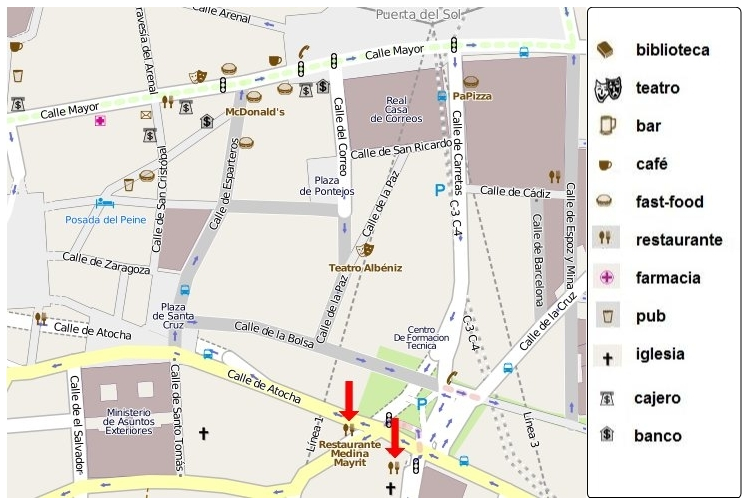
\includegraphics[width=\textwidth]{images/corpus/mapa10.png}\\[0pt]
\caption{Imagen sin zoom, target plural}
\label{mapa-zoom-plural}
\end{figure}


En la Tabla \ref{freq-mapa-zoom-plural} se muestran las ER, la cantidad de ocurrencia en el corpus


\begin{table}[H]
{\footnotesize
\begin{center}
\begin{tabular}{|l|c|c|c|c|}
\hline
ER 					      & Cantidad &  Frecuencia & SubE & SobreE\\ \hline \hline
Medina Mayrit y el que esta cerca        &	11	&	\% & NO & NO \\ \hline
el de la calle Atocha y De La Cruz       &	3  &	\%	&SI & NO\\  \hline
pr\'oximo a la iglesia 	      &1		&	\%	&SI &\\ \hline
Medina Mayrit y el que esta en Calle De Atocha	      &5		&	\%	&SI&NO\\ \hline
Calle De Atocha				&	2  &	\%	&SI&NO\\ \hline
Restaurantes de Calle De Atocha				&	8  &	\%	&SI&NO\\ \hline
Medina Mayrit en Calle de Atocha y el que esta cerca				& 3  &	\%	&NO&SI\\
cerca de la iglesia				&	  &	\%	&&\\ \hline
Medina Mayrit			&11		&	\%	&SI&NO\\  \hline
Medina Mayrit y el que esta cerca				&	1	&	\%  &NO&SI\\
en la calle Atocha y De La Cruz        &	  &	&&\\ \hline
El que esta en Calle De Atocha y Carretas, 	      &		&	\%	&NO&NO\\
y el de Atocha y de la Cruz	      &1		&	&&\\ \hline
El que esta en Calle De Atocha y Carretas 					&	2  &	\%	&SI&NO\\ \hline
Medina Mayrit en Calle De Atocha y el que esta cerca  				&  1 &	\%	&NO&SI\\ \hline
Medina Mayrit y el que esta cerca				&		3 &	\%  &NO &SI\\
cercano a la iglesia				&	  &	&&\\ \hline
Medina Mayrit y el que esta 	&	2	&	\%  &NO&SI\\
cerca de la iglesia				&	  &	&&\\ \hline
Medina Mayrit en Calle de Atocha y el que esta cerca			&1  &	\%	&NO&SI\\
en Calle De La Cruz	&	  &		&&\\ \hline
Medina Mayrit y el que esta cerca			&1  &	\%	&NO&SI\\
en Calle De Atocha	&	1  &		&&\\ \hline
Medina Mayrit y el que esta cerca			&2  &	\%	&NO&SI\\
en Calle De La Cruz	&	  &		&&\\ \hline
Calle De Atocha y Calle De La Cruz  					&1  &	\%	&SI&NO\\
\hline \hline
Totales	&	&	100\%	&&\\

\hline
\end{tabular}
\caption{ER del corpus dadas por humanos para el mapa de la Figura \ref{mapa-zoom-plural}.}\label{freq-mapa-zoom-plural}
\end{center}
}
\end{table}




Para el mapa de la Figura \ref{mapa-zoom-plural} el vocabulario y probabilidades de uso de las palabras es el siguiente:

Restaurante 62/65=0.95\\
MedinaMayrit 48/65=0.738\\
ProxA 41/65 = 0.63\\
CalleDeAtocha  33/65=0.507\\
Iglesia 17/65=0.261\\
CalleDeLaCruz 11/65 = 0.169\\
CalleDeCarretas 4/65=0.061\\
in = 36/65 =0.554\\


El modelo coincide con el modelo de la Figura \ref{modelo-mapa-zoom}, ya que es el mismo mapa.

%rest4 near rest3
%rest4 in CalleDeAtocha
%str15 CalleDeCarretas
%str16 CalleDeLaCruz

%Las probabilidades de uso de las palabras y el vocabulario se muestran a continuaci\'on:
%
%ParroquiaDeSantaCruz 66/73=0.904
%in 23/73=0.315
%CalleSantoTomas 22/73=0.301
%CalleDeAtocha 4/73=0.055
%CalleDeLaConcepcionJeronima 7/73=0.096
%church 6/73=0.082
%near 6/73=0.082
%MinisterioDeRelacionesExteriores 5/73=0.068 (notar que no esta en el modelo!)
%

%\begin{figure}[ht]
%\centering
%\begin{tikzpicture}
  %[
    %n/.style={circle,fill,draw,inner sep=5pt,node distance=4cm},
    %aArrow/.style={scale=10,->, >=stealth, thick,
    %shorten <= 1pt, shorten >= 1pt},
  %]
			%
%
	%\node[n,label=left:$str17$,label=below:{
    %\relsize{-2}$\begin{array}{c}
     %\nStreet\end{array}$}] (a) {};		
			%
	%\node[n,label=above:$str12$,label=below:{
    %\relsize{-2}$\begin{array}{c}
      %\nStreet\\[-3pt] 
      %\nCalleDeElSalvador\end{array}$}, right of=a] (b) {};
  %
	%\node[n,label=left:$str16$,label=below:{
    %\relsize{-2}$\begin{array}{c}
      %\nStreet\\[-3pt] 
      %\nCalleDeLaCruz\end{array}$}, right of=b] (m) {};		 
%
%\node[n,label=below:$str10$,label=above:{
    %\relsize{-2}$\begin{array}{c}
      %\nStreet\\[-3pt] 
      %\nCalleSantoTomas\end{array}$}, above of=b] (c) {};	
				%
 %\node[n,label=left:$min1$,label=above:{
    %\relsize{-2}$\begin{array}{c}
      %\nBuilding\\[-3pt] 
      %\nMinAsExt\end{array}$}, above of=a] (f) {};	
					%
  %\node[n,label=left:$church1$,label=below:{
    %\relsize{-2}$\begin{array}{c}
     %\nChurch\end{array}$}, above of=f] (g) {};
			%
 %\node[n,label=left:$church2$,label=below:{
    %\relsize{-2}$\begin{array}{c}
     %\nChurch\end{array}$}, right of=c] (d) {};
			%
  %\node[n,label=below:$rest3$,label=above:{
    %\relsize{-2}$\begin{array}{c}
      %\nRestaurante\\[-3pt] 
      %MedinaMayrit\end{array}$}, above of=d] (h) {};			
			%
 %\node[n,label=below:$str9$,label=above:{
    %\relsize{-2}$\begin{array}{c}
      %\nStreet\\[-3pt] 
      %\nCalleAtocha\end{array}$}, above of=c] (e) {};		
%
%\node[n,label=left:$rest4$,label=below:{
    %\relsize{-2}$\begin{array}{c}
      %\nRestaurante\end{array}$}, right of=m] (k) {};
%
%\node[n,label=above:$d$,label=below:{
    %\relsize{-2}}, right of=d] (i) {};
		%
 %\node[n,label=below:$str15$,label=above:{
    %\relsize{-2}$\begin{array}{c}
      %\nStreet\\[-3pt] 
      %\nCalleDeCarretas\end{array}$}, above of=i] (j) {};	
%
%%\node[n,label=below:$str17\nStreet$,label=above:{
 %%   \relsize{-2}}, below of=k] (n) {};				
 %\draw [aArrow,<->,bend right=40] (g) to node[auto,swap]{\relsize{-3}$\nFrenteCerca$} (f);
%% \draw [aArrow,bend right=40] (f) to node[auto,swap]{\relsize{-3}$\nFrenteCerca$} (g);
%
 %\draw [aArrow,bend right=40] (g) to node[auto,swap]{\relsize{-3}$\nIn$} (c);
 %\draw [aArrow,bend right=20] (g) to node[auto,swap]{\relsize{-3}$\nIn$} (e);
%
 %\draw [aArrow,bend right=40] (d) to node[auto,swap]{\relsize{-3}$\nIn$} (m);
 %\draw [aArrow,<->,bend right=-10] (d) to node[auto,swap]{\relsize{-3}$\nFrenteCerca$} (i);
 %%\draw [aArrow,bend right=40] (i) to node[auto,swap]{\relsize{-3}$\nFrente$} (d);
 %\draw [aArrow,<->,bend right=40] (k) to node[auto,swap]{\relsize{-3}$\nCerca$} (d);
 %%\draw [aArrow,bend right=40] (d) to node[auto,swap]{\relsize{-3}$\nCerca$} (k);
 %\draw [aArrow,<->,bend right=80] (k) to node[auto,swap]{\relsize{-3}$\nCerca$} (h);
%
 %\draw [aArrow,bend right=40] (k) to node[auto,swap]{\relsize{-3}$\nIn$} (m);
 %\draw [aArrow,<->,bend right=20] (k) to node[auto,swap]{\relsize{-3}$\nFrenteCerca$} (i);
%% \draw [aArrow,bend right=40] (i) to node[auto,swap]{\relsize{-3}$\nFrente$} (k);
 %\draw [aArrow,bend right=20] (h) to node[auto,swap]{\relsize{-3}$\nIn$} (e);
 %\draw [aArrow,bend right=-20] (h) to node[auto,swap]{\relsize{-3}$\nIn$} (j);
%
 %\draw [aArrow,bend right=30] (f) to node[auto,swap]{\relsize{-3}$\nIn$} (c);
 %\draw [aArrow,bend right=40] (f) to node[auto,swap]{\relsize{-3}$\nIn$} (e);
 %\draw [aArrow,bend right=40] (f) to node[auto,swap]{\relsize{-3}$\nIn$} (a);
 %\draw [aArrow,bend right=40] (f) to node[auto,swap]{\relsize{-3}$\nIn$} (b); 
%
 %\draw [aArrow,bend right=5] (i) to node[auto,swap]{\relsize{-3}$\nIn$} (e);
 %\draw [aArrow,bend right=40] (i) to node[auto,swap]{\relsize{-3}$\nIn$} (m);
%%\draw[dotted] (-0.5,-1.1) rectangle (10.5,3.1);
%
 %\end{tikzpicture}
%\caption{Grafo del contexto \ref{mapa-zoom}}
%\label{modelo-mapa-zoom-plural}
%\end{figure}




















\section{Notas finales y linkeo del cap\'itulo}
%%%%%%%%%%%%%%%%%%%%%%%%%%%%%%%%%%%%%%%%%%%%%%%%%%%%%%%%%%%%%%%%%%%%%%%%%%%%%%%%%%%%%%%%%%%%%%%%%%%%%%%%%%%%%%%%%%%%%%%%%%%%%%%%%%%%%%%%%%%%%%%%%%%%%%%%%%	       >2
\label{sec-final}

%This paper has introduced the Zoom corpus of natural language descriptions of map locations. The corpus takes into account a domain that is significantly closer to real-world applications, and addresses more complex situations of reference than existing resources of this kind. In particular, the Zoom domain makes use of  contexts with different levels of detail, and contains instances of singular and plural reference produced by a relatively large number of speakers in both Spanish and Portuguese languages.

%Preliminary results of a SVM-based approach to GER - which were solely presented for the future assessment of GER algorithms based on Zoom data - hint at the actual complexity of the GER task in this domain in a number of ways. 

%First, we notice that a similar SVM-based approach in \cite{thiago-svm} on GRE3D3 and GRE3D7 data has obtained considerably higher mean accuracy (0.46 and 0.64 respectively) and higher mean Dice scores (0.78 and 0.89 respectively). This is of course explained by the increased complexity of the Zoom domain (e.g., in number of objects and possible atomic and relational properties etc.). However, we notice also that the Zoom annotation scheme - although taking into account an already large number of possible attributes - is still overly simple. In particular, the attribute {\em others} has been overused and, as a result, the chances of reproducing the corpus descriptions is narrow. Clearly, more work needs to be done to expand the annotation scheme and split {\em others} into a larger number of attributes.

%Second, Zoom descriptions are prone to convey relations between a single target and multiple landmark objects, as in `the restaurant on 5th street, near the library'. Although common in language use, the use of multiple relational properties in this way has been little investigated, perhaps because it may lead to ambiguous descriptions, as in `the restaurant near the church on Jackson street and the bar on 5th street' for a restaurant located near the junction of these two streets.

%As future work, we intend to make the corpus publicly available for research on multiple aspects of content selection and surface realisation in REG. In particular, we envisage the use of the Zoom corpus as training and test data for machine learning models of REG, and also to address further issues that have not been addressed in the present paper. These include  the generation of referring expressions from knowledge bases with different degrees of detail, and the issues of between-speakers and within-speakers variation in REG.

%En este cap\'itulo se ha presentado el corpus de zoom de las descripciones en lenguaje natural de localizaciones en el mapa. 
En este cap\'itulo vimos como se recolect\'o el corpus Zoom, los materiales que se usaron para la recolecci\'on estan en Ap\'endice \ref{corpus-apendice}, la anotaci\'on del corpus, el an\'alisis y evaluaci\'on del mismo. 

para que?\\
Este corpus se cre\'o viendo la necesidad de existencia de recursos en dominios m\'as naturales. Se recolect\'o mediante un experimento on-line en el que las personas ve\'ian un mapa el cual conten\'ia una o dos flechas indicando el o los targets y completaban una ER dirigida a un amigo en la cual ten\'ian que describir el o los objetos sen\~alados. Cada persona di\'o 20 ER 10 singulares y 10 plurales, de esas 10 singulares o plurales, hab\'ia 5 con alto nivel de zoom y 5 con bajo nivel de zoom.

El corpus tiene en cuenta un dominio que es significativamente m\'as cerca de aplicaciones del mundo real, y aborda las situaciones m\'as complejas de referencia de los recursos existentes de este tipo nombrados en el Cap\'itulo \ref{sec:corpus2}. En particular, el dominio de zoom hace uso de contextos con diferentes niveles de detalle, y contiene ejemplos de referencia singular y plural producido por un n\'umero relativamente grande de hablantes en ambos idiomas espa\~nol y portugu\'es, siendo el lenguaje seleccionado el lenguaje nativo de la persona.

analisis respecto a ER que contiene\\
En este corpus podemos encontrar distintos tipos de ER como las nombradas en \ref{sec:seleccion}, tenemos varias ER por mapa con lo cual podremos luego calcular las probabilidades de uso de las palabras como se explic\'o en \ref{sec:learning} para ejecutar nuestro algoritmo explicado en el Cap\'itulo \ref{sec:algoritmo}. Dadas las caracter\'isticas de los mapas usados para la recolecci\'on, el corpus tiene ER relacionales, proposicionales, de plurales, sobre-especificadas y hasta under-especificadas.

analisis respecto a la anotacion\\
El corpus fue anotado por 2 personas y finalmente un juez decidi\'io cual anotaci\'on dejar, la anotaci\'on se hizo teniendo en cuenta atributos para el target tipo, nombre, en (refiri\'endose a donde est\'a, en que calle), relaciones espaciales (izquierda, derecha, en esquina / entre, cerca, en-frente-de, detr\'as) estas relaciones requer\'ian la ER de otros objetos (landmarks), en algunos caso solo uno, y en otros 2, y el \'ultimo atributo disponible fue {\it otro}, para anotar cosas que no se hab\'ian tenido en cuenta en la anotaci\'on nombrada. Para cada uno de los landmarks se tuvieron en cuenta 4 atributos m\'as, con lo que para cada ER tenemos un m\'aximo de 26 atributos o relaciones cuando el target era singular y 52 cuando el target era plural. El atributo {\it otro} nos ayuda en el sentido de que podemos agrupar las ER que solo difieren en este atributo, pero nos juega en contra ya que esas ER que contienen {\it otro} no las podremos generar, es decir perdemos parte de la informaci\'on que la persona di\'o. Se midi\'o el porcentaje de acuerdo (kappa) entre los jueces y fue del 84\%. 

evaluacion\\ (no se si dejar esta parte aca, o pasar la evaluacion esta al cap 6)

Se realiz\'o una evaluaci\'on cuyos resultados preliminares de un enfoque basado en SVM a GER - que fueron \'unicamente presentados para la futura evaluaci\'on de algoritmos GER basados en datos Zoom - alusi\'on a la complejidad real de la tarea GER en este dominio.

En primer lugar, nos damos cuenta de que un enfoque basado en SVM similar en~\cite{thiago-svm} en datos de GRE3D3 y GRE3D7 ha obtenido considerablemente mayor precisi\'on media (0,46 y 0,64 respectivamente) y una mayor media de las puntuaciones de Dice (0,78 y 0,89 respectivamente). Esto, por supuesto, se explica por el aumento de la complejidad del dominio Zoom (por ejemplo, en el n\'umero de posibles objetos y propiedades at\'omicas y relacionales etc.). 

Sin embargo, nos damos cuenta tambi\'en que el esquema de anotaci\'on Zoom  aunque teniendo en cuenta ya gran n\'umero de posibles atributos - sigue siendo demasiado simple. En particular, el atributo {\em otro} ha sido usado en exceso y, como consecuencia, las posibilidades de reproducci\'on de las descripciones corpus es pequen\~a. Es evidente que a\'un queda trabajo por hacer para ampliar el esquema de anotaci\'on y dividir lo que se anot\'o como {\em otros} en un mayor n\'umero de atributos.

En segundo lugar, las descripciones de zoom son propensas a transmitir las relaciones entre un solo objeto y varios objetos emblem\'aticos, como en `el restaurante en la calle 5, cerca de la biblioteca '. Aunque es com\'un en el uso del lenguaje, el uso de m\'ultiples propiedades relacionales de esta manera ha sido poco investigado, tal vez debido a que puede dar lugar a descripciones ambiguas, como en `el restaurante cerca de la iglesia en la calle Jackson y el bar en la calle 5' para un restaurante situado cerca del cruce de estas dos calles.

Como trabajo futuro, tenemos la intenci\'on de hacer que el corpus quede a disposici\'on p\'ublica para la investigaci\'on sobre m\'ultiples aspectos de la selecci\'on de contenidos y la realizaci\'on de superficie en GER. En particular, prevemos el uso del corpus zoom como datos de entrenamiento y prueba de modelos de aprendizaje autom\'atico de GER, y tambi\'en para abordar otras cuestiones que no se han abordado en el presente trabajo. Estos incluyen la generaci\'on de expresiones referenciales de bases de conocimiento con diferentes grados de detalle aprovechando que el corpus tiene esa caracter\'istica, y las cuestiones de la variaci\'on entre los hablantes y del mismo hablante en GER.

%\section{Conclusiones y linkeo del cap\'itulo}

 

